\documentclass[hyp]{socreport}
\usepackage[ruled,vlined]{algorithm2e}
\usepackage{amsmath}
\usepackage{graphicx}
\usepackage{subcaption}
\graphicspath{ {./images/} }
\usepackage{fullpage}
\begin{document}
\pagenumbering{roman}
\title{Warehouse Optimisation Using Quadratic Assignment on New Hardware}
\author{Xu Jun}
\projyear{2019/2020}
\projnumber{H074910}
\advisor{A/P Wong Weng Fai, Dr Luo Tao}
\deliverables{
	\item Report: 1 Volume
	}
\maketitle
\begin{abstract}
As quantum computing gains traction, there is a significant effort in applying it to real-world problems. One of the approaches is to use quantum annealing for the Quadratic Assignment Problem (QAP), which in turn has a wide range of applications. The strategy is to convert a QAP into Quadratic Unconstrained Binary Optimisation(QUBO) form which is compatible with hardware solver.

However, the number of binary variables in QUBO is quadratic with respect to the size of the generating QAP. This leads to a lack of scalability in state-of-the-art quantum(-inspired) annealers. 

This project explores a novel heuristic that overcomes such scalability issue for a special class of QAPs satisfying a block-structural property. This property is frequently observed in practical settings such as warehouse allocation. The heuristic enables quantum(-inspired) annealers to solve block-structural QAPs of sizes linear to the number of physical qu-bits.

The heuristic is explored on two platforms, the D-Wave 2000Q Quantum Annealer (QA) and the Fujitsu Digital Annealer (DA).

Experiments are performed on standard datasets as well as in-house block-structural QAP instances, and performance comparison is made against traditional, software simulated annealing.

Results demonstrate that the hardware platforms, with the new heuristic, produce solutions of comparable quality on standard datasets and are superior on in-house instances. Moreover, the hardware solutions achieve significant speedups. It is claimed that quantum(-inspired) annealers, with the help of the new heuristic, can be used to solve QAPs to good effect.


\begin{descriptors}
    \item C5 Computer System Implementation
\end{descriptors}
\begin{keywords}
	Quadratic Assignment Problem, Quadratic Unconstrained Binary Optimisation, Application-specific Hardware, Simulated Annealing
\end{keywords}
\begin{implement}
	Macintosh OS, IBM ILOG CPLEX Optimisation Studio, Python 3.6
\end{implement}
\end{abstract}

\listoffigures 
\listoftables
\tableofcontents 

\chapter{Introduction}
\label{ch:intro}
2.The workings of quantum annealing hardware
3.The issue of scalability in quantum hardware

\section{QAP for Warehouse Optimisation}
This section starts with general warehouse optimisation and subsequently introduces QAP.

\subsection{General warehouse assignment}

Consider the problem of assigning items to locations in a warehouse. How should the assignment be done, so that when orders come in and items are picked, the travel distance of the picker is at a minimum? For a company, the reduction of such distance translates to the reduction of labour cost. That is the significance of the problem and the motivation for initiating this project.

\label{sec:example}
The objective is to find a decent storage assignment policy to minimise travel distance for a given set of orders. There exist many assignment policies. Below is an example from Tsige \cite{Tsige:2013} reproduced to illustrate them. 

The example is set up as follows. Suppose a warehouse has layout as in Fig 1.1. It is a rectangular warehouse, with three aisles and 30 slots in total. Each aisle can reach to two columns to the left and the right. There is an Input/Output (I/O) point at the bottom left corner through which items are transported in and out.
\begin{figure}
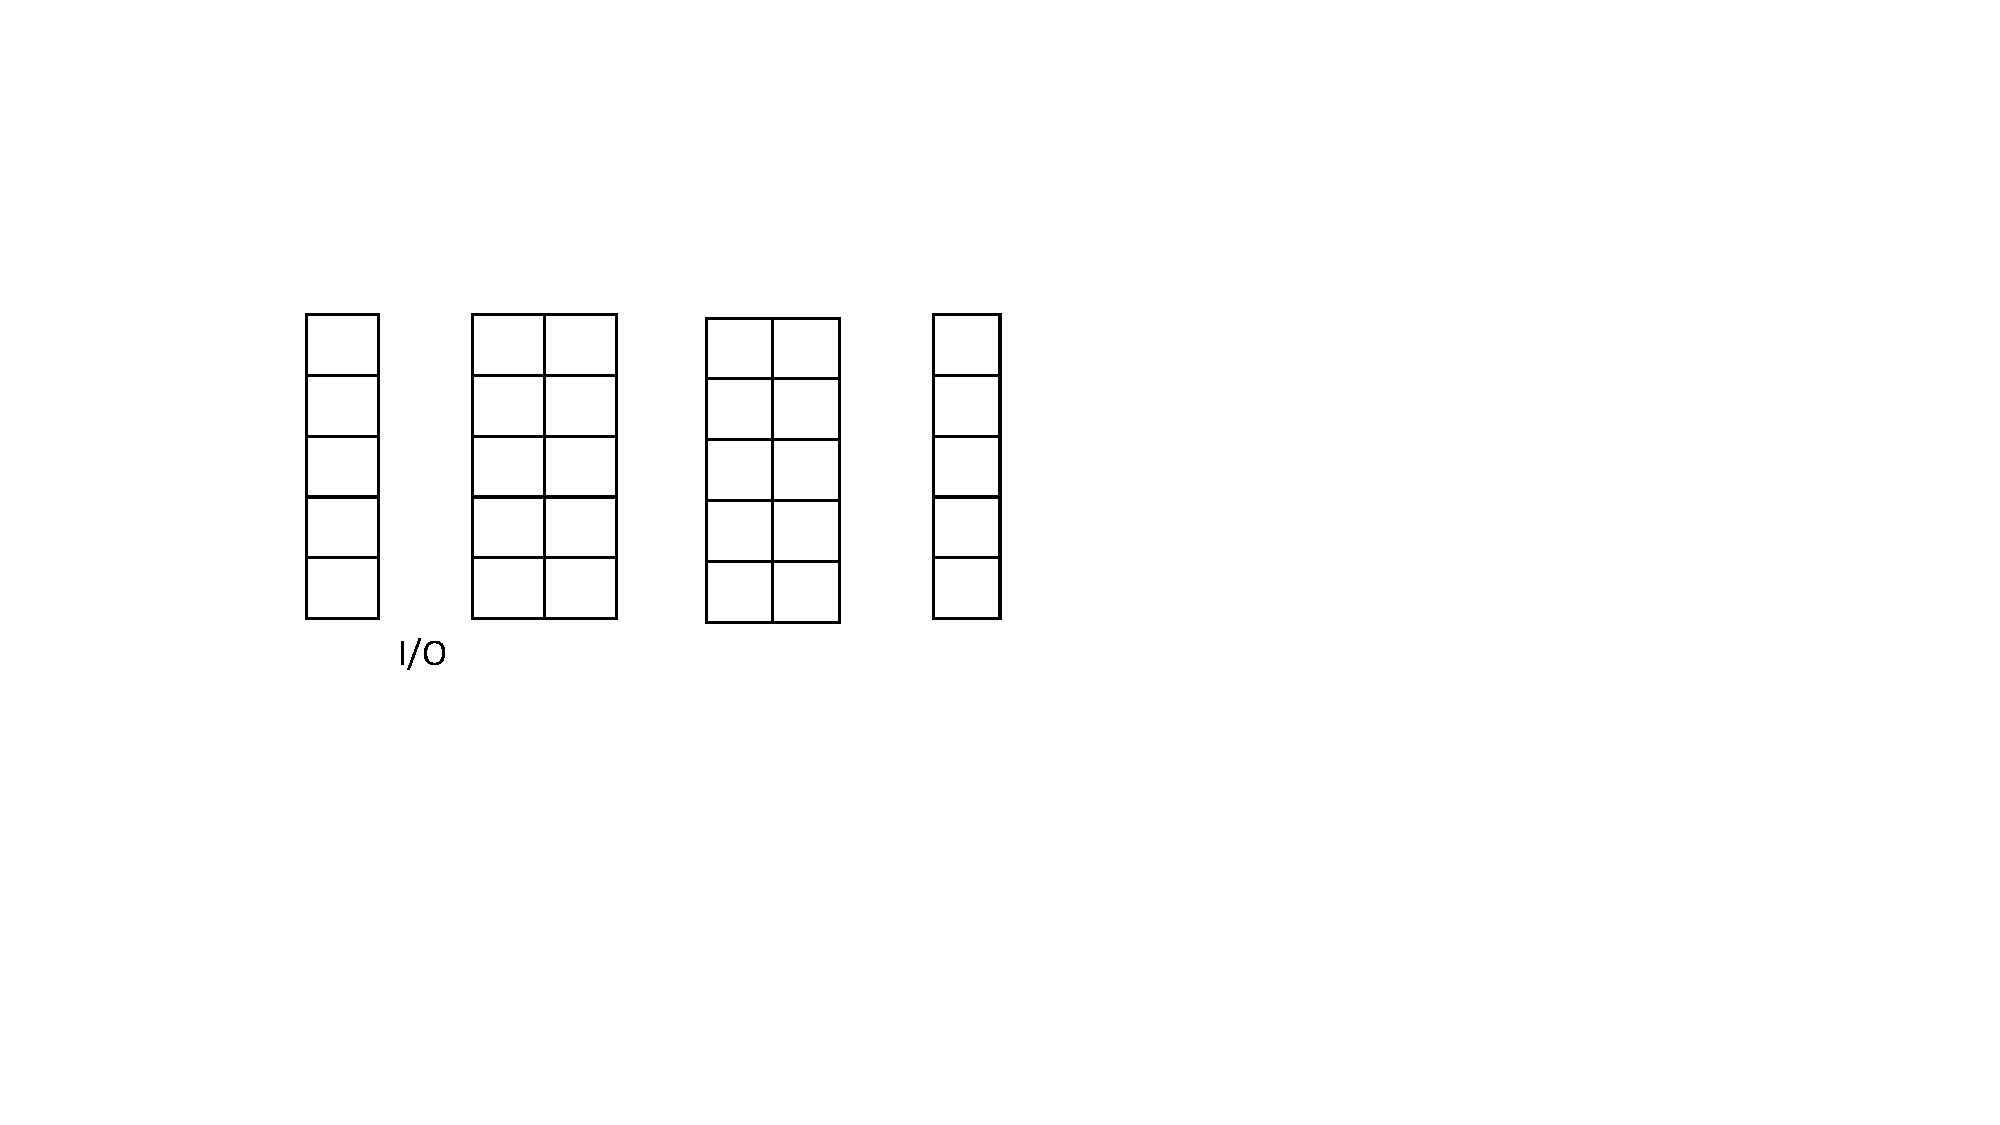
\includegraphics[scale=0.8]{empty}
\centering
\caption{layout of an empty warehouse}
\end{figure}

\begin{figure}
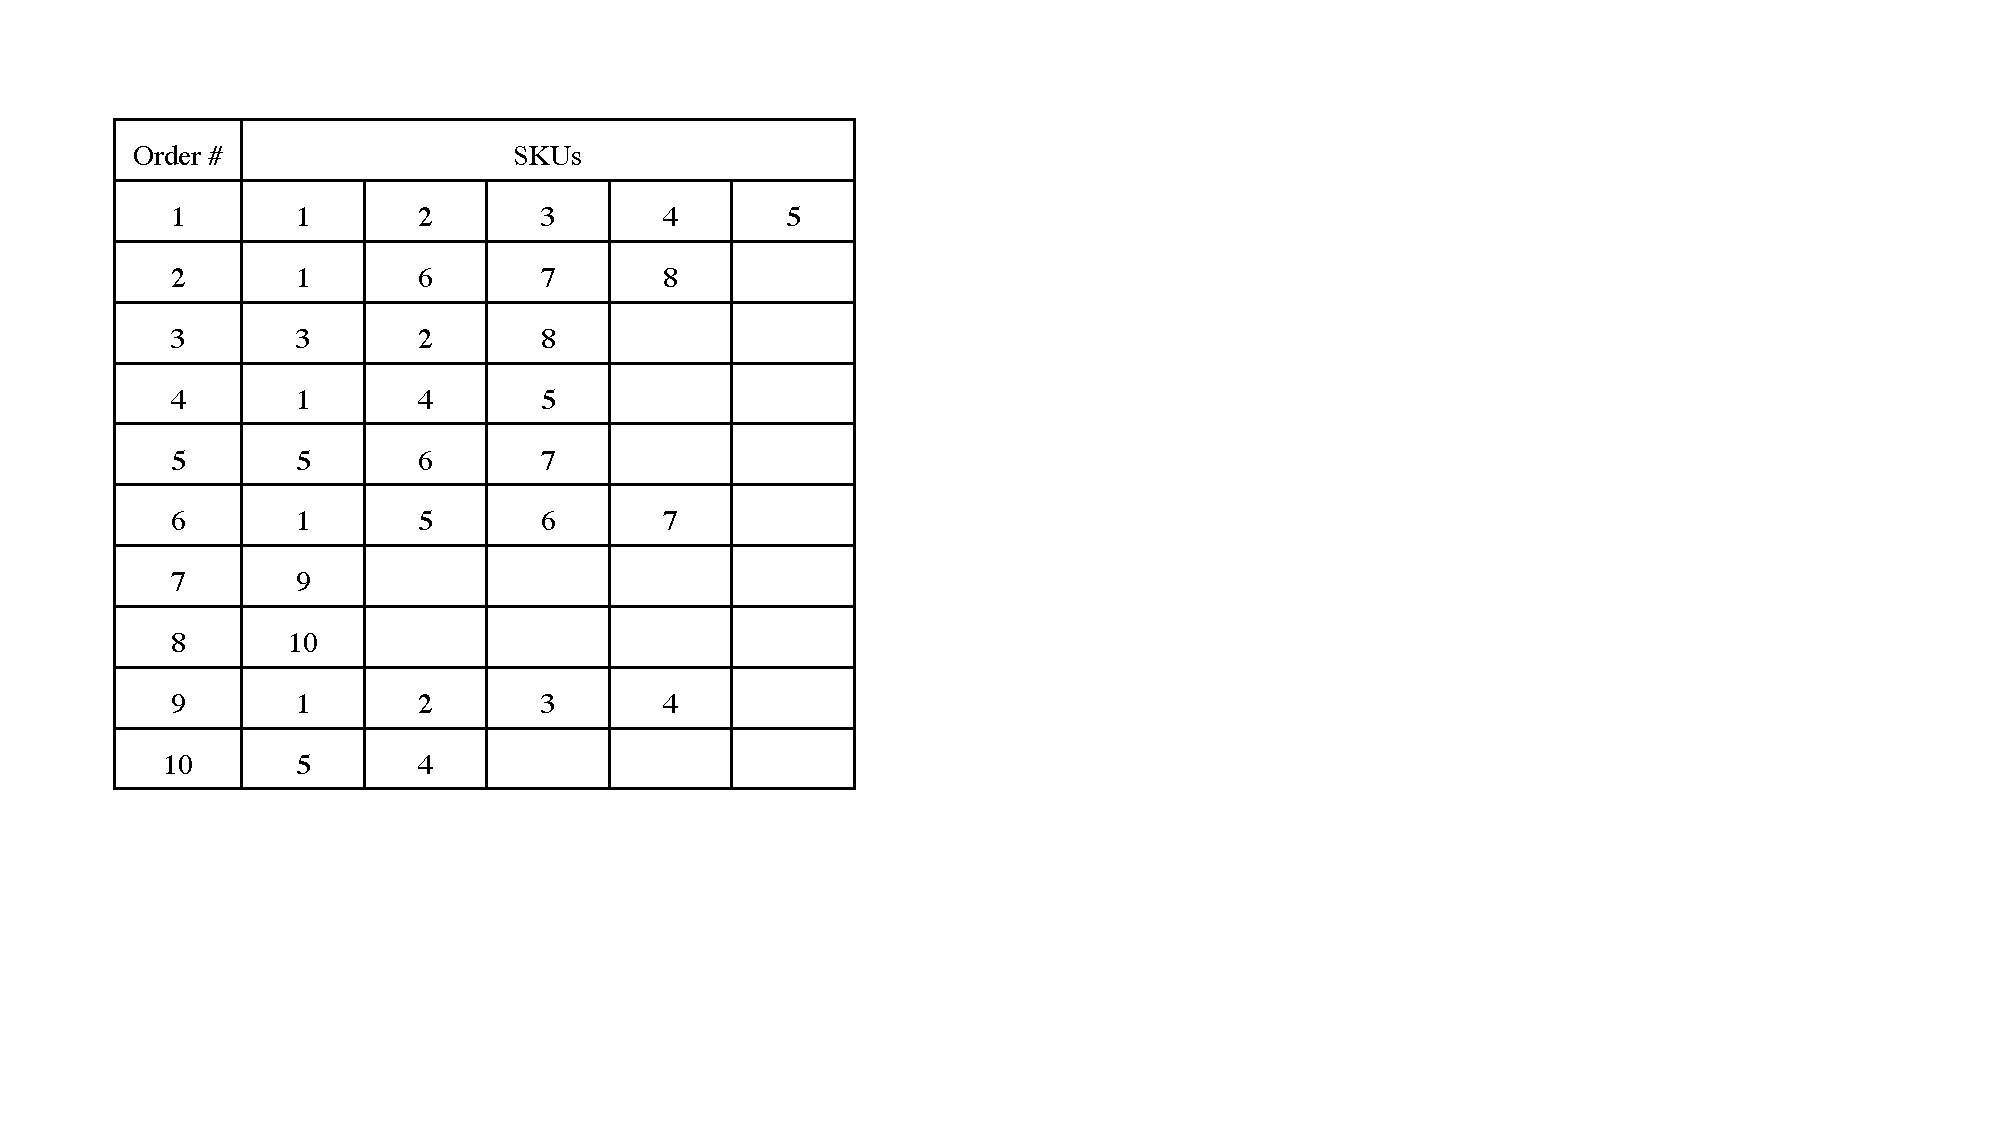
\includegraphics[scale=0.7]{orders}
\centering
\caption{the set of orders}
\label{fig:orderset}
\end{figure}

Next, there is a set of orders as described in Fig 1.2. There are 10 orders and a total of 10 Storage Keep Units (SKUs) associated with the orders. An SKU is a type of items. Note that there are in total 30 items appearing in the order set. The correct number of items of each type need to be assigned.

In general, to pick an order, the picker starts from the I/O point. According to a fixed routing strategy, he travels around the warehouse collecting the needed items and travels back to the I/O point after all items in the order are collected.

Traditionally, there are various warehouse assignment strategies. A few of them are described below.

\textbf{Dedicated storage} always assigns items to their own locations in the warehouse. This means every item has its dedicated location. This policy then relies on order pickers' memory power to minimise travel distance.

\textbf{Random storage} assigns items randomly. An instance is shown in Fig \ref{fig1.3:a}.

\textbf{ABC storage} groups SKUs into classes according to popularity and allocates a dedicated area for each class. The number of popularity classes and the number of items in each class are arbitrary. For example, in Fig\ref{fig1.3:b} we have around 20\%, 40\% and 40\% of items in classes A,B,C respectively, up to minor adjustments of discrete numbers. SKU 1 is the most popular and items of SKU 1 all fall into class A. Subsequently, SKUs 2,4,5 go to class B. The rest goes to class C. Next, count the number of locations required for each class and assign a dedicated area for the class. For example, class A requires 5 locations and gets an area at closest Euclidean distance to the I/O point.

\textbf{Cube-per-order(COI) storage} assigns items according to their ratio between volume and popularity. For the interest of this project, we consider all items to have identical volume so this reduces to arranging items according to popularity. An example is shown in Fig \ref{fig1.3:c}.

\subsection{Motivation for order-oriented strategies}
ABC and COI policies are product oriented. That is, they rely on historical data about each specific product, such as popularity. Intuitively, they optimise average distance in picking a set of \textit{individual} items. If each order contains only a single item, then these policies might achieve a good average distance reduction. On the other hand, they do not take into account the \textit{structure} of any particular order. Order structure is crucial because each order has several items picked together and, on a conceptual level, the shortest distance in picking the entire order is different from the shortest average distance in picking a set of individual items. This is the motivation for order-oriented policies, for which Mantel coined the term Order-Oriented Slotting (OOS) \cite{Mantel:2007}. In his terms, policies such as ABC and COI are \textit{single-command} strategies that are unfit for order picking, which is a \textit{multiple-command} situation. The goal of OOS is to take a set of orders and directly model and minimise travel distance based on the set. Section \ref{sectionQAP} is dedicated to this type of strategies. In particular, order-oriented swapping and QAP are introduced.

\begin{figure}
\begin{subfigure}{.5\textwidth}
	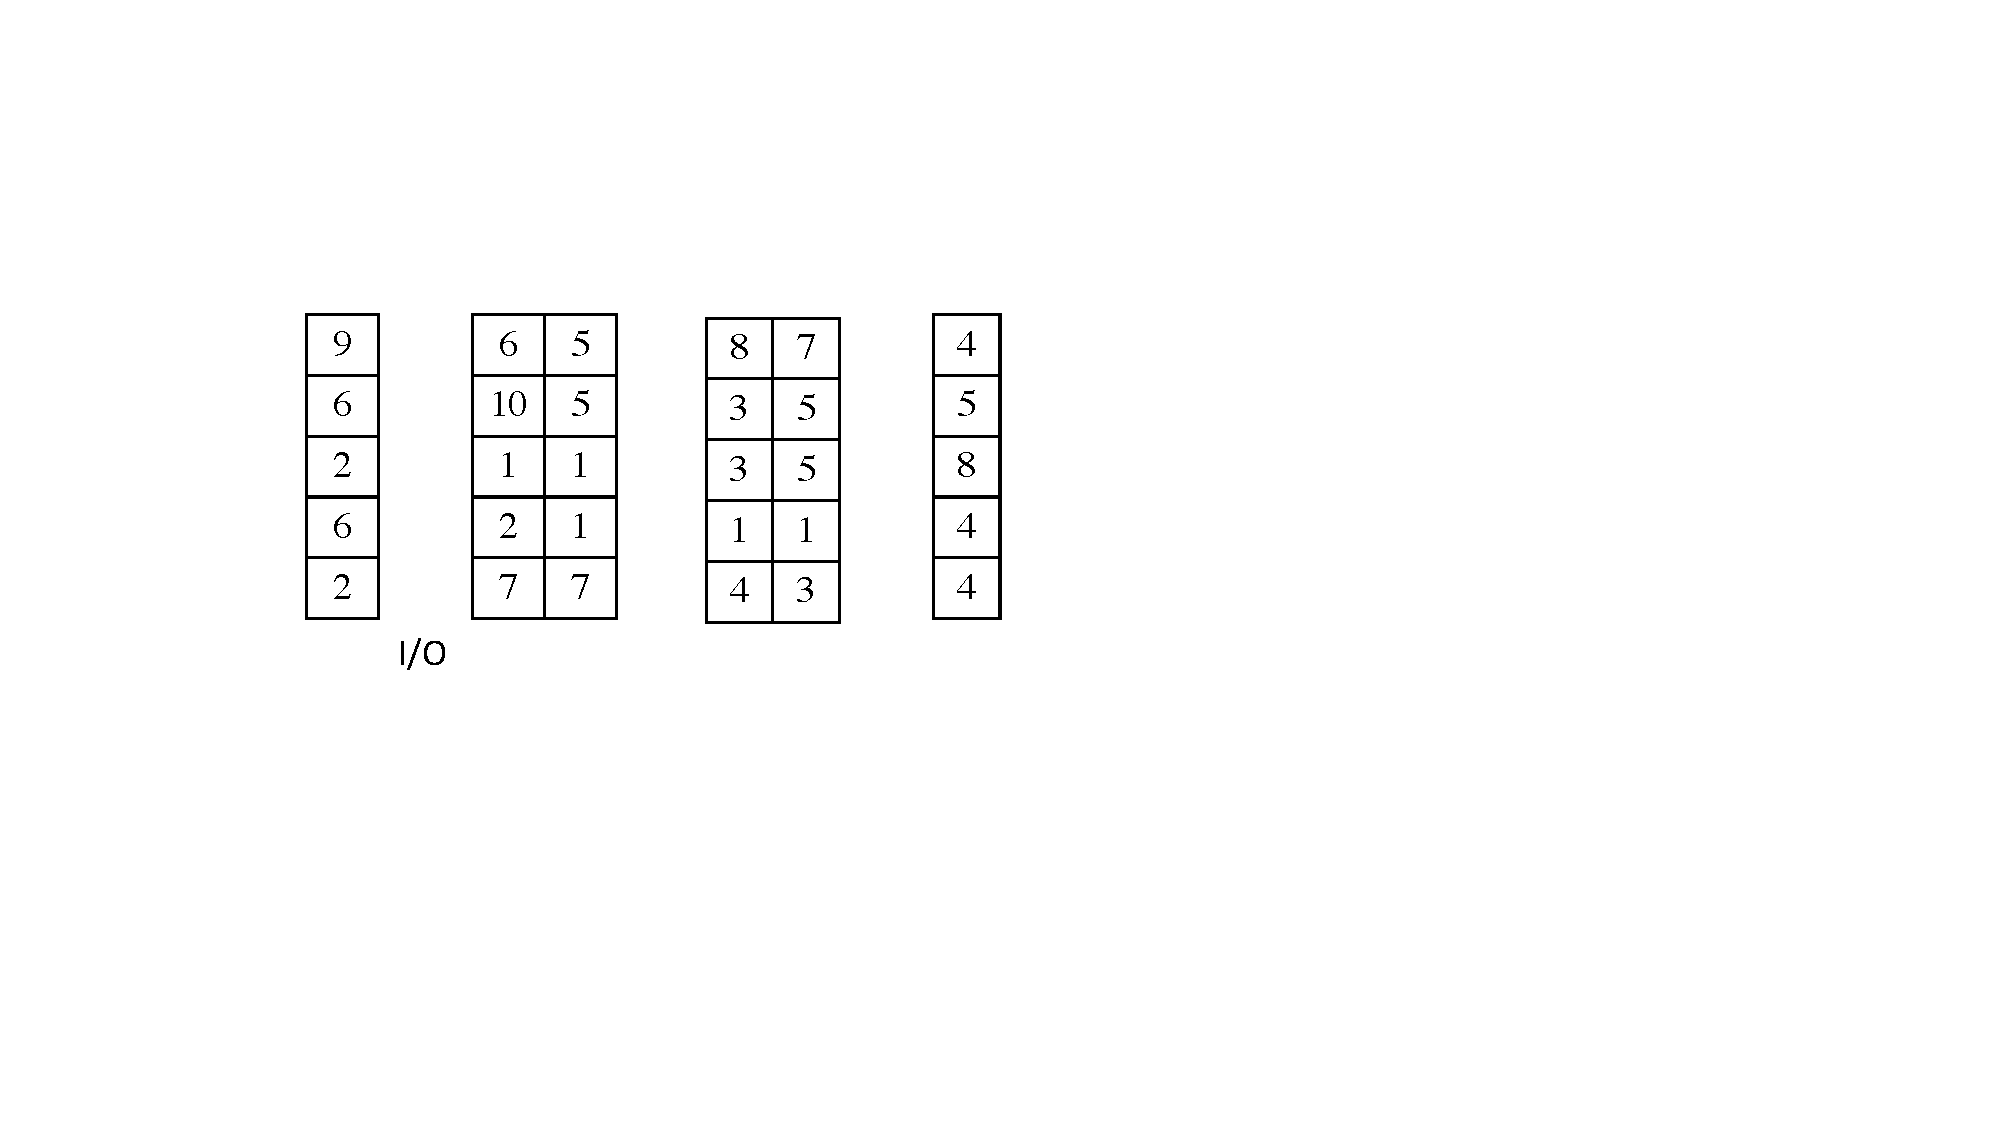
\includegraphics[scale=0.5]{random}
	\centering
	\caption{random}
	\label{fig1.3:a}
\end{subfigure}
\begin{subfigure}{.5\textwidth}
	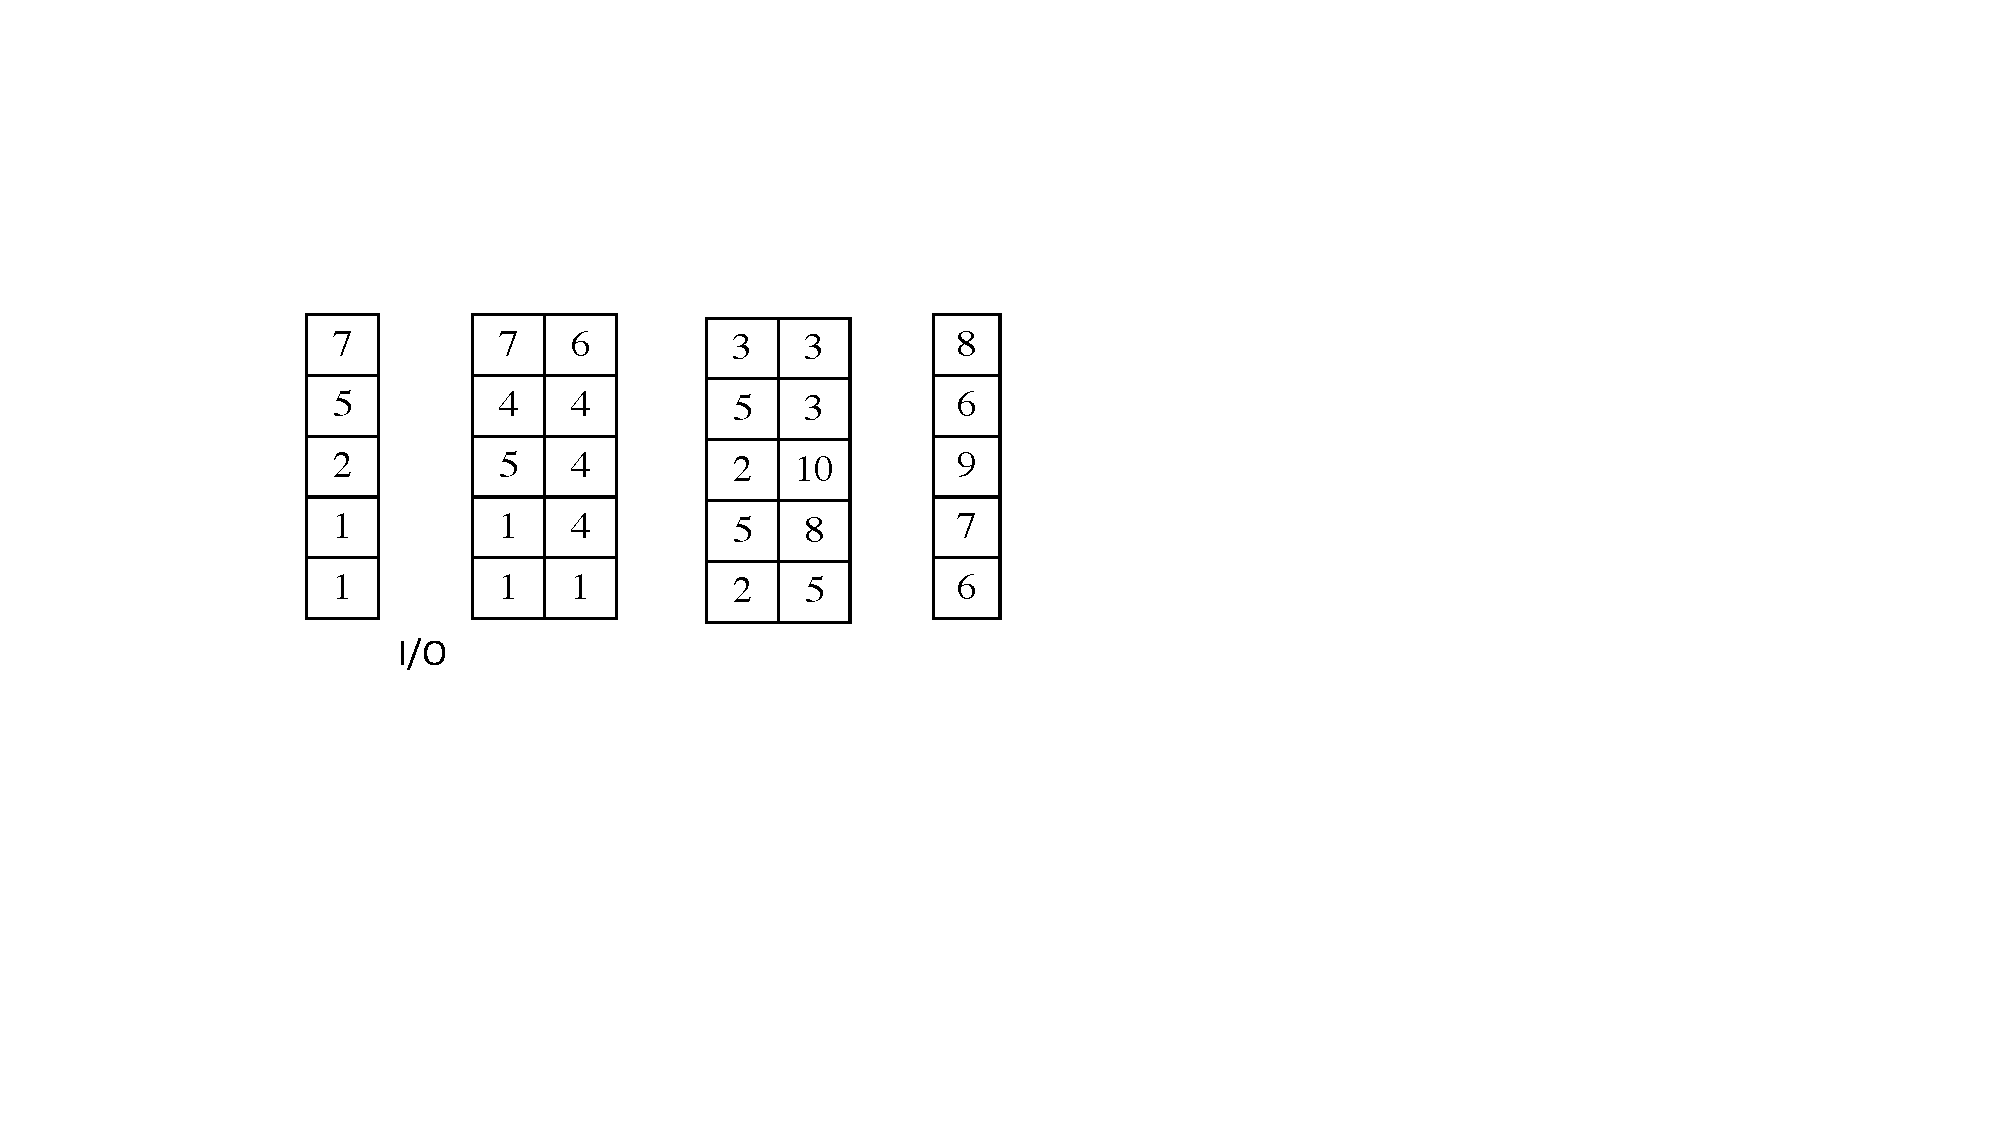
\includegraphics[scale=0.5]{abc}
	\centering
	\caption{ABC}
	\label{fig1.3:b}
\end{subfigure}
\begin{subfigure}{.5\textwidth}
	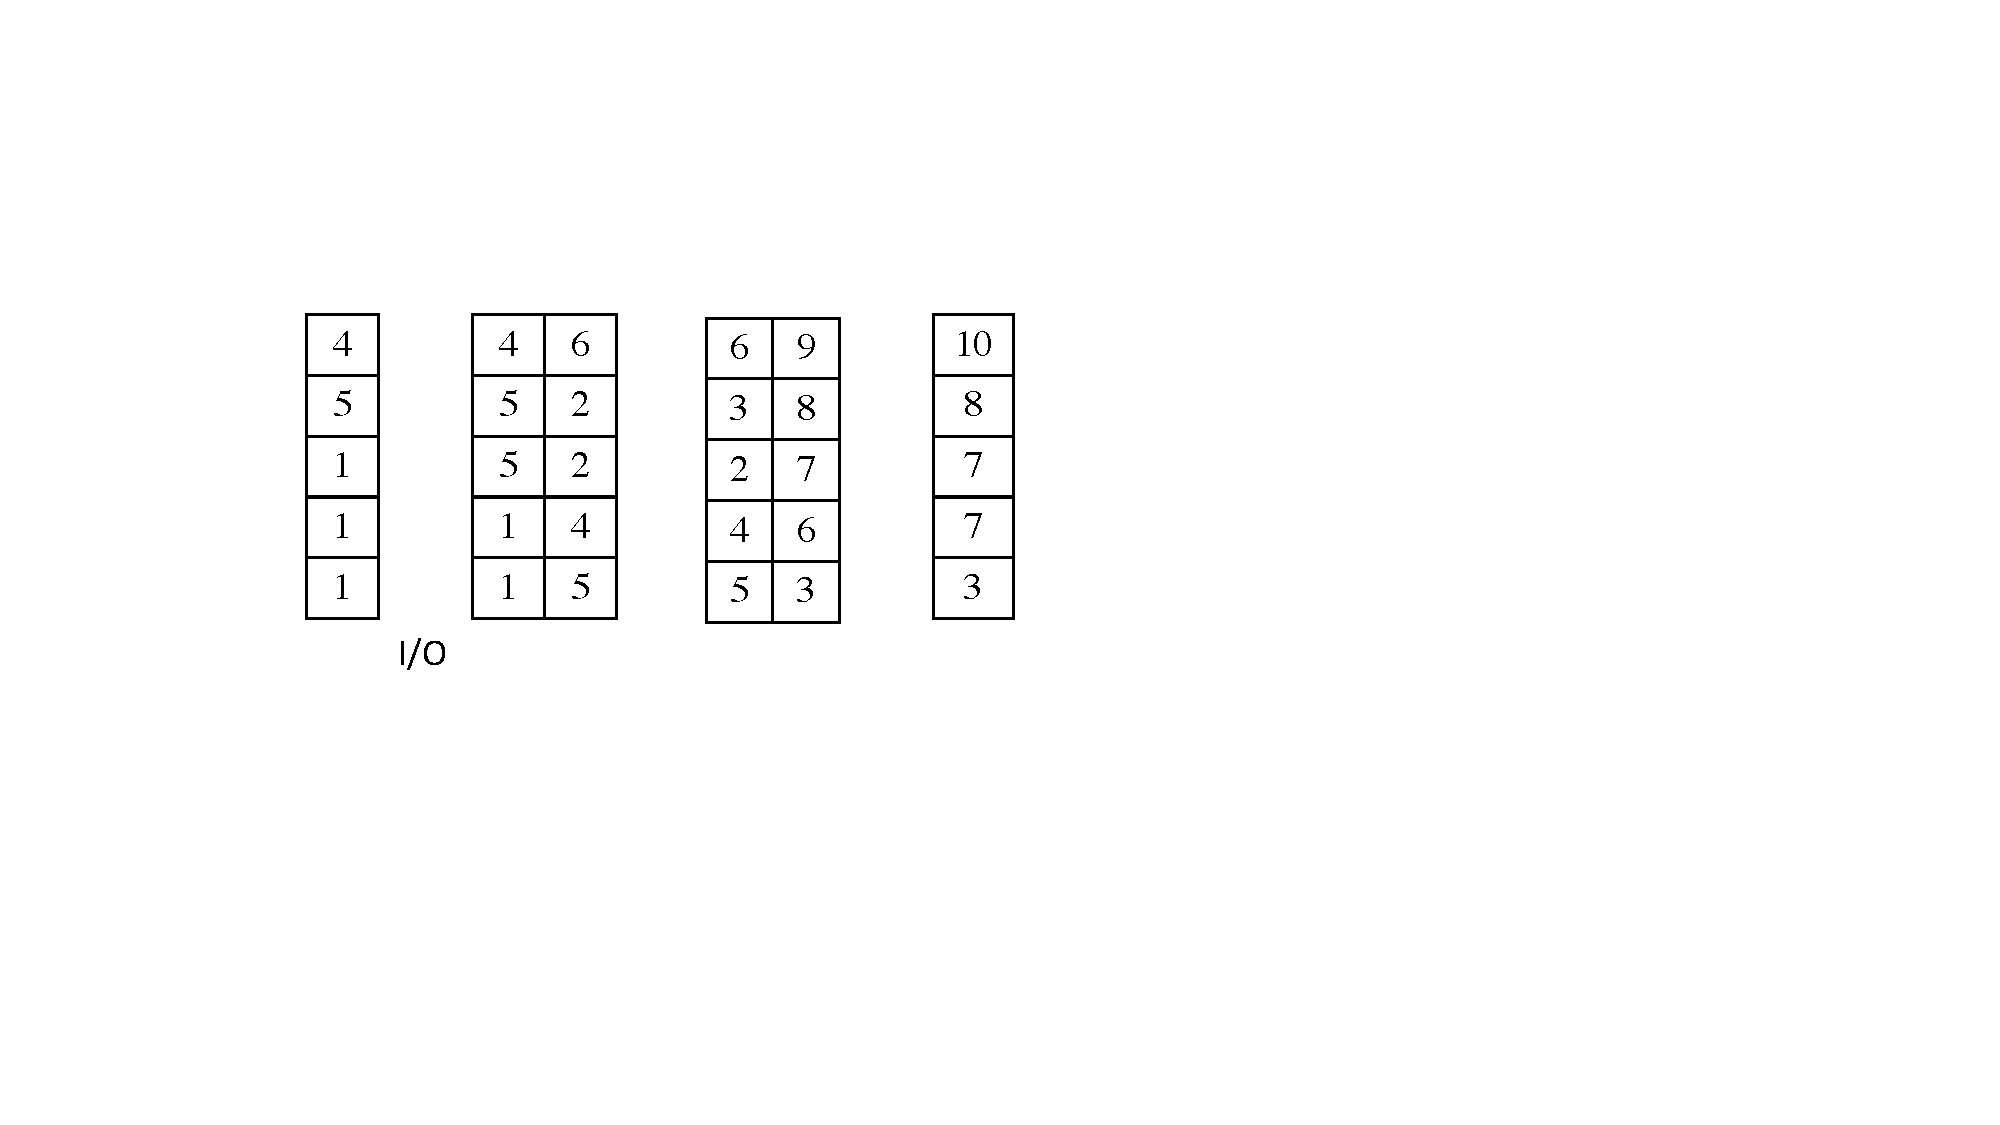
\includegraphics[scale=0.5]{coi}
	\centering
	\caption{COI}
	\label{fig1.3:c}
\end{subfigure}
\begin{subfigure}{.5\textwidth}
	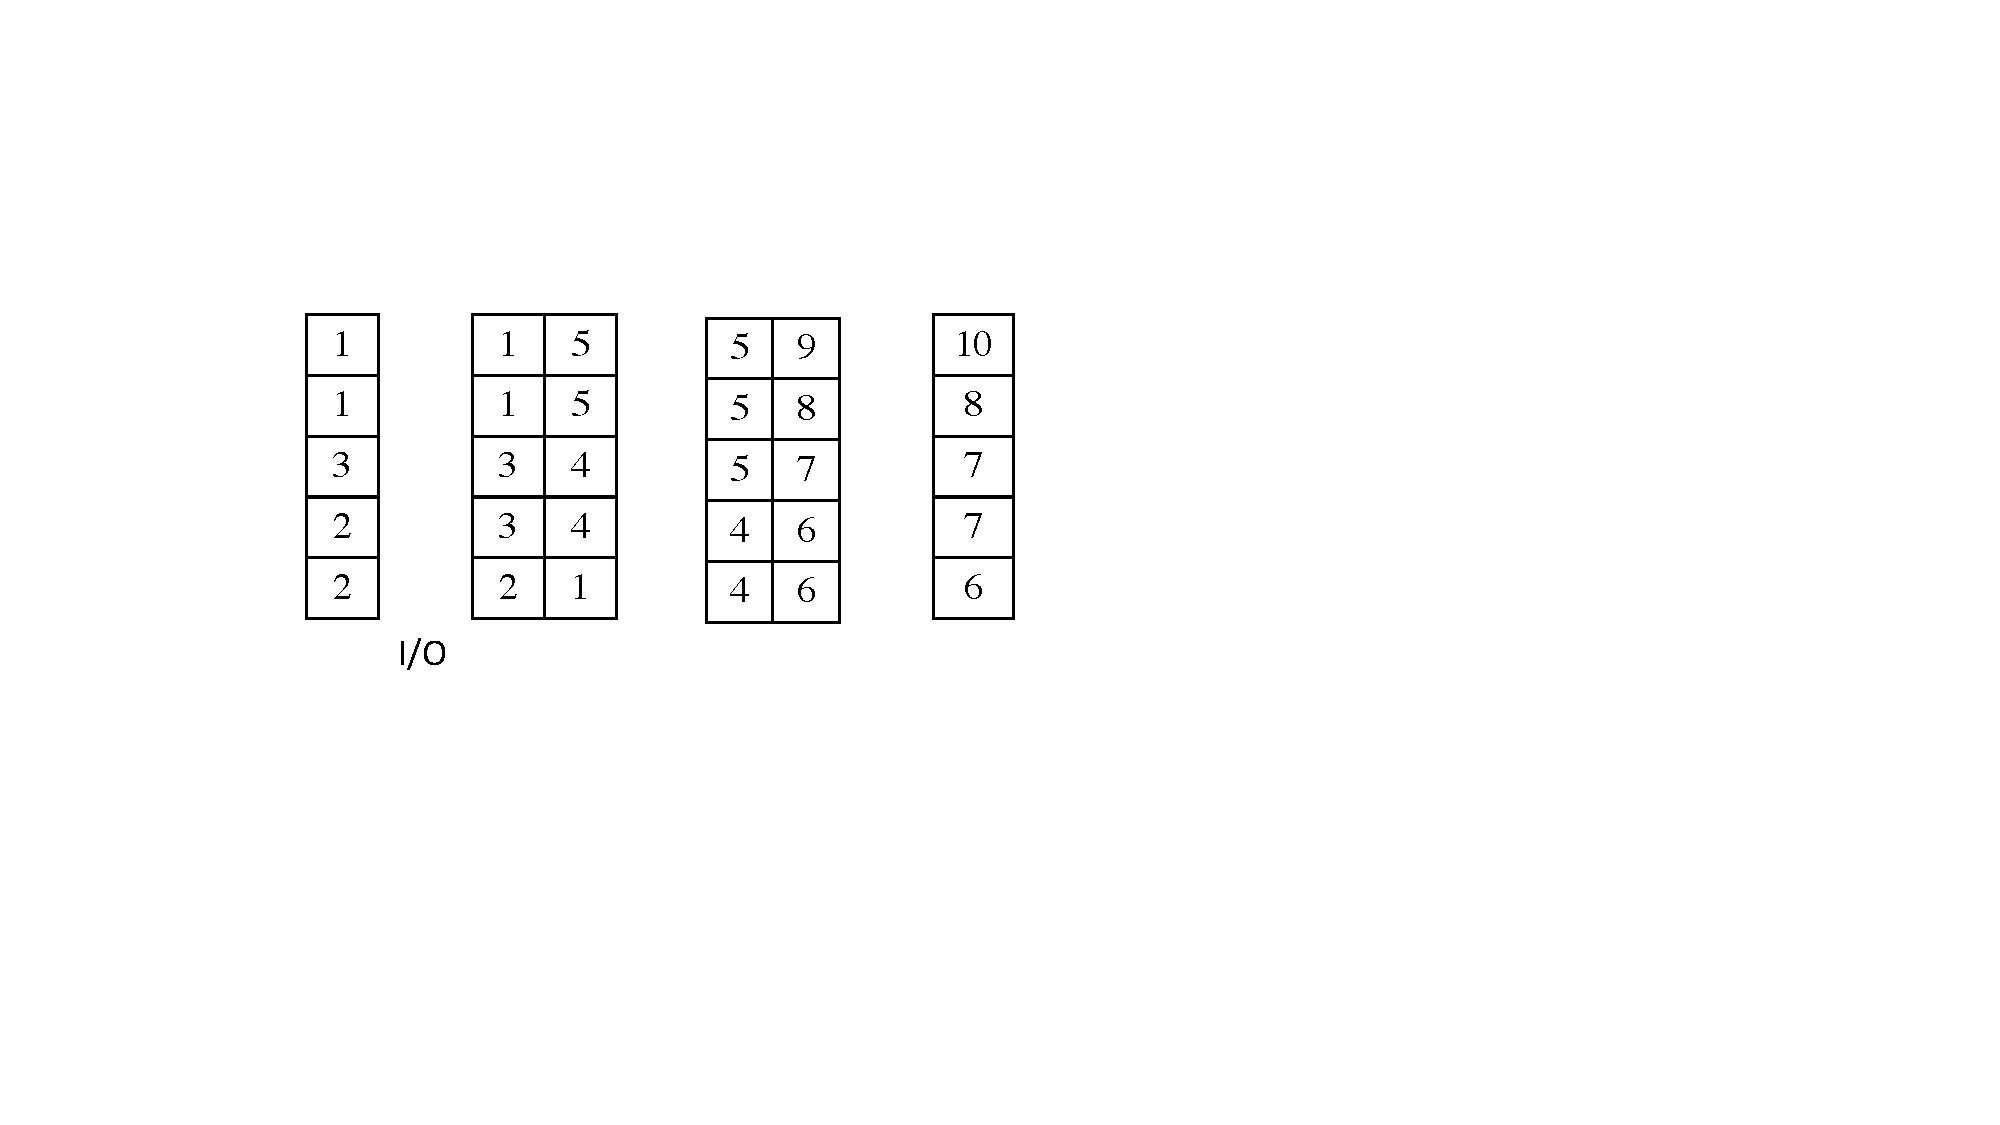
\includegraphics[scale=0.5]{ifh-oos}
	\centering
	\caption{Order-oriented swapping (OOS)}
	\label{fig1.3:d}
\end{subfigure}
\caption{storage layout after assignment}
\label{fig:variouslayouts}
\end{figure}

\section{Order-oriented strategies}
\label{sectionQAP}
Suppose there is an order set $O$. To calculate distance travelled in picking $O$, a routing policy needs to be determined. Next, according to this routing policy, distance travelled for picking each order in $O$ can be computed, and distance travelled in picking $O$ is the sum of distance for each order. Altogether, the problem is of the form $(O,R)$ where $O$ denotes the order set and $R$ denotes the routing policy.

Overall, this type of problems is called Combinatorial Optimisation problems.
\subsection{Routing policy}
For simplicity, S-shaped routing policy is assumed throughout the text. S-shaped routing has the following characteristics.

1) The picker starts from the I/O point

2) The picker identifies the two end columns of items in the order

3) The picker identifies every column in which there is item to be picked

4) The picker travels horizontally to the leftmost column which contains an item to be picked

5) The picker traverses every column in which there is item to be picked

6) There is no change of direction within a column

\begin{figure}
	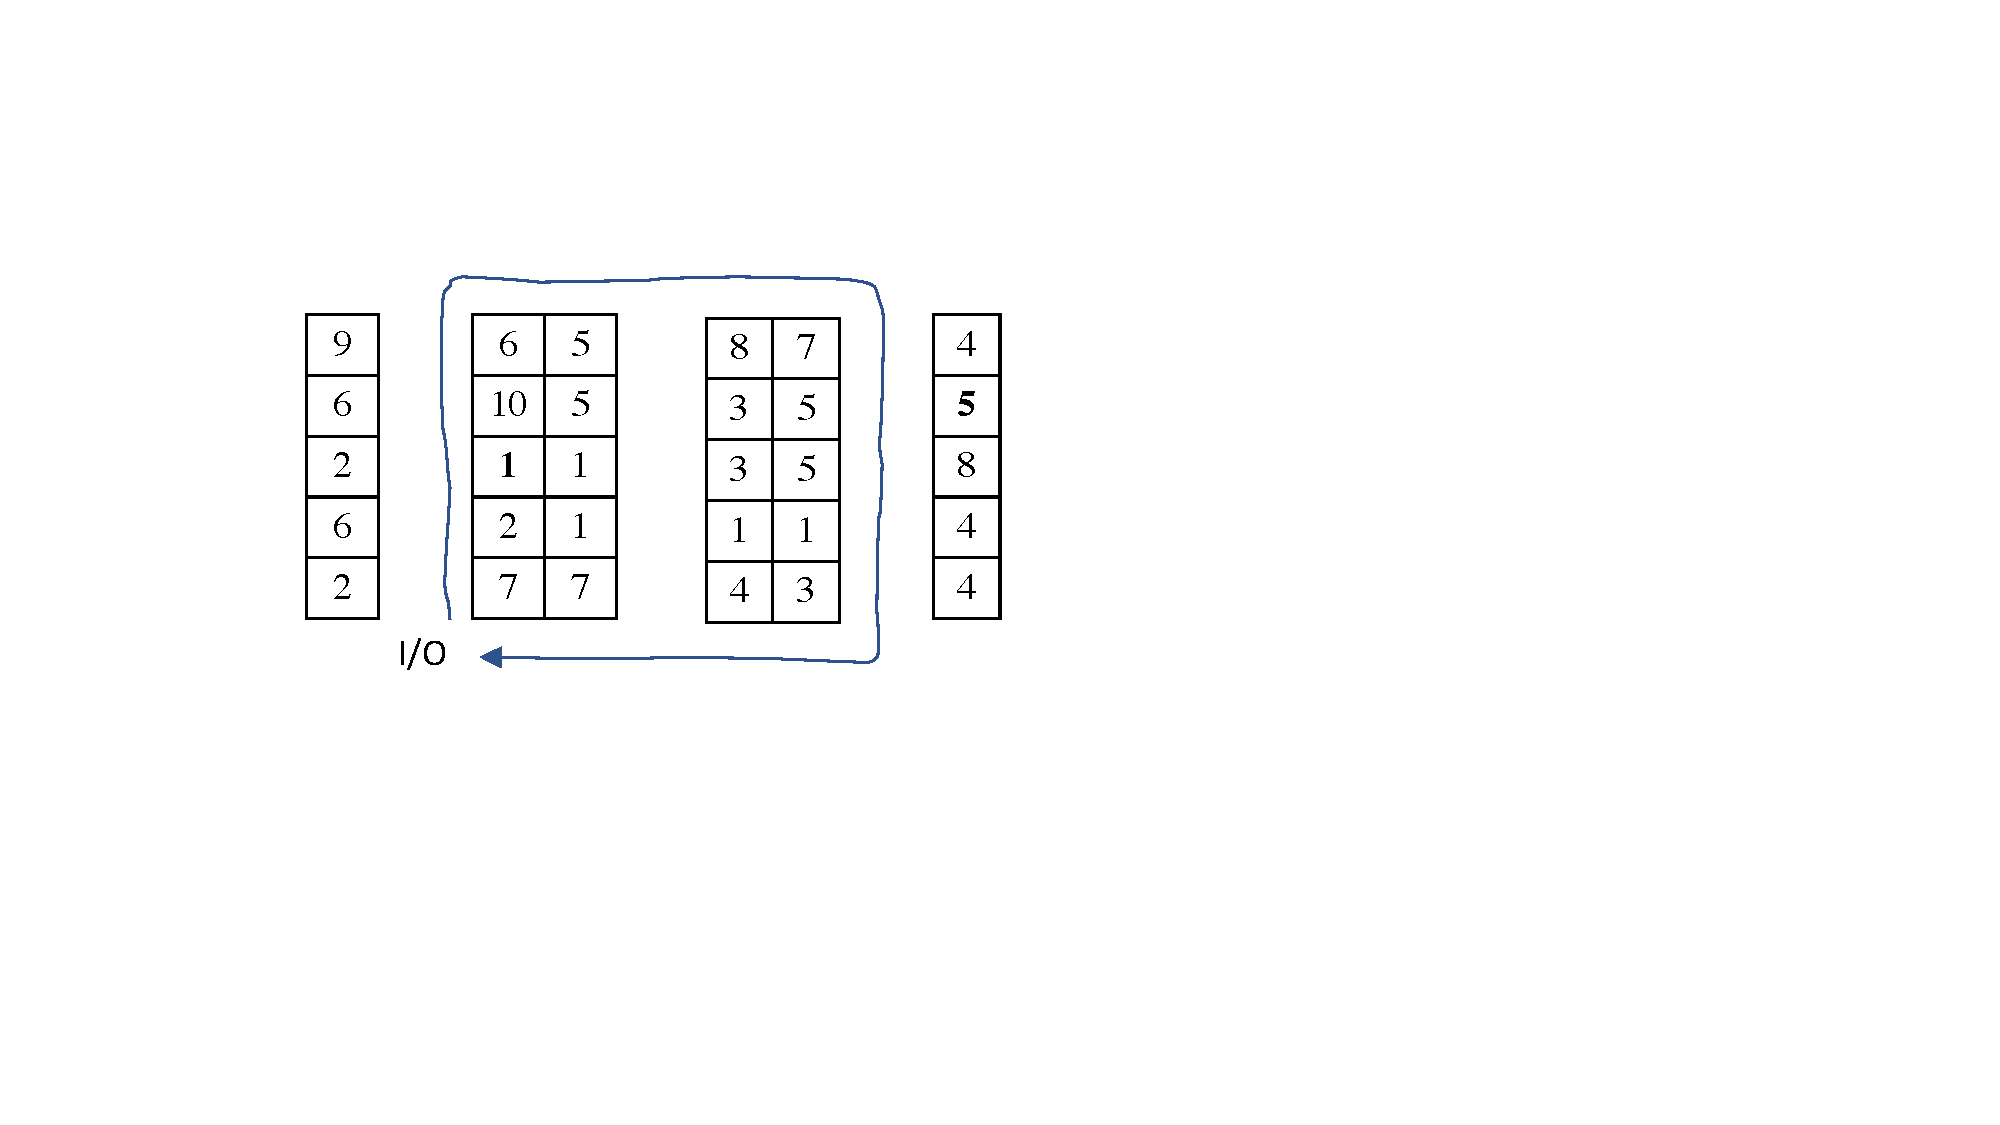
\includegraphics[scale=0.8]{routing}
	\centering
	\caption{S-shape routing}
	\label{fig1.4}
\end{figure}

An example to illustrate the idea is shown in Fig \ref{fig1.4}. SKU 1 in the first column and SKU 5 in the third column are picked. The picker traverses the first and the third columns and skips the middle column.

There are more routing policies other than S-shaped. However, it is difficult to incorporate more complicated routing policies into the strategy. The reason is that an assignment strategy would often utilise the concept \textit{routing-based distance} to compute travelled distance, which means assignment depends on routing. Sophisticated routing policies, on the other hand, might depend on assignment. This creates a cyclic dependence between routing policy and assignment strategy to which a solution is hard to find. Therefore, simple S-shaped routing, which is independent of assignment, is used by the strategies introduced later in this section.

\subsection{Simulated annealing}
There are many ways to solve combinatorial optimisation problems. Exact solution methods such as branch-and-bound exist, but normally take too long to be useful. Practically, heuristics are employed to discover suboptimal but decent solutions. Normally, a heuristic is only developed for a specific problem instance and cannot be used across the board. However, a special kind of heuristics, the metaheuristics, arise in recent years and shed light on the generic way the solution space of any combinatorial optimisation problem is searched. One of them is Simulated Annealing (SA), which imitates the physical process of how a piece of hot metal anneals, i.e. cools down naturally to minimal energy. In the optimisation problem, the energy of metal corresponds with the formula that is to be minimised. It is postulated that after several iterations, the solution yielded by SA would be of decent quality.

The high level idea of SA is that at each temperature, several randomly generated, neighbouring new \textit{states} are explored. If the new \textit{state} is better (with lower energy), it is accepted and replaces the current one. Otherwise, the new state is accepted with a probability given by the Metropolis criterion:
\[p = exp^{\frac{-\Delta E}{T}}\]
where $\Delta E$ is the change in energy and $T$ is the current temperature. This occasional acceptance of a worse state (with higher energy) is crucial because the overall state would then avoid being trapped in a local minimum. After a number of trials, the temperature is lowered by multiplying with a cooling factor $\alpha$. The entire procedure ends when some target temperature is reached. The pseudocode of SA is shown below.

\singlespacing
\begin{procedure}[H]
\SetAlgoLined
\KwResult{Near optimal solution}
 param TARGET\_T\{target temperature\}\;
 param NT\{number of attempts within a single temperature\}\;
 param $\alpha$ \{cooling factor\}\;
 $t = t_0$\{starting temperature\}\;
 $p = p_0$\{starting state\}\;
 $e = E(p_0)$\{starting energy\}\;
 $p_{best} = p$\;
 $e_{best} = e$\;
 k = 0\;
 
 \While{t $>$ TARGET\_T}{
	\For{n from 1 to NT}{
		$p_{new} = random(p)$\{randomly generate a new solution\}\;
		$e_{new} = E(p_{new})$\;
		$\Delta E = e_{new} - e$\;
		$prob = exp^{\frac{-\Delta E}{t}}$\;
		\If{$\Delta E$ is less than zero}{
			$p = p_{new}$\;
			$e = e_{new}$\;
		}
		\ElseIf{$prob > random(0,1)$}{
			$p = p_{new}$\;
			$e = e_{new}$\;
		}
		\If{$e < e_{best}$}{
			$p_{best} = p$\;
			$e_{best} = e$\;
		}
	}
 	$t = t\times \alpha$ \;
 }
 $return (p_{best}, e_{best})$\;
 \caption{Simulated Annealing()}
\end{procedure}
\normalspacing
\bigskip
One may wonder how the parameters are obtained for a specific problem. In fact, the best parameters are determined empirically. The set of parameters is called a \textit{cooling schedule}. There exist cooling schedule proposals that seem to work well for combinatorial optimisation problems.

\subsection{Order-oriented swapping (OOS)}
Order-oriented swapping is a simulated annealing technique developed by Ruijter \cite{Ruijter:2007}. It basically takes the problem $(O,R)$ and instantiates the SA procedure with the following correspondences:

1) state := assignment policy

2) energy := \textit{$R$-specific} distance travelled in picking $O$

The reason this technique is called \textit{swapping} is that the way of generating new solutions is in fact swapping two random items in the current assignment.

As specified in simulated annealing, every iteration requires computing the new energy $e_{new}$. This is the most computationally intensive step in the entire algorithm because it involves iterating through $O$ and accumulating distances from scratch. That is the reason Ruijter found that even though this method yields solutions of good quality, it takes a rather long time to finish and is therefore impractical. The result of running this strategy is shown in Fig \ref{fig1.3:d}.

\subsection{The strategy of QAP}
\label{sec:qap}
The Quadratic Assignment Problem (QAP) is a well-known combinatorial optimisation problem. It has the following statements. There are $n$ facilities and $n$ locations. Between any two facilities there are products transported to and fro, and the amount of transport is called \textit{flow}. Between two locations there is some distance. Define \textit{traffic} as the product of flow and distance. How to assign facilities to locations such that the total traffic is minimised?

The most important concept that inspires the application of QAP in warehouse assignment is the heuristic that if two SKUs frequently appear together in the same order (higher \textit{flow} between two SKUs), then items of those SKUs should be assigned closer to each other (lower \textit{distance} between assigned locations). Intuitively, this would reduce the amount of \textit{traffic} in picking orders because the picker is most likely to spend minimal distance in between items appearing in an order. As a side note, the QAP strategy preserves the benefit of COI in that it requires more popular items to be assigned closer to the I/O point.

The QAP is outlined as follows. There are $n$ locations and $n$ items. Between each pair of items there is a \textit{flow} indicating the frequency of them appear in the same order. Note that flow is initially defined for pairs of SKUs, not pairs of items. Here, define the flow between items to be the value of the flow between their respective SKUs.

Additionally, between each pair of locations there is a distance. Note that this distance is \textit{routing-specific}. With S-shaped routing, the distance between two items is proportional to the number of columns between them, since the picker would in principle traverse those columns in a zig-zag manner. However, during actual picking the picker would skip a column if there is no item to be picked in that column, hence this distance is approximate. For example, in Fig \ref{fig:diffdist}, different situations result in different distances between items 1 and 5. In \ref{fig:routingskip}, there is no item to be picked in the middle so distance is approximately 2 columns' length. In \ref{fig:routingthrough}, item 3 has to be picked, so middle column has to be traversed and distance between 1 and 5 becomes 3 columns' length. It is assumed throughout the report that all columns in between are traversed when computing distance. We have arrived at the following formal formulation of QAP.

\begin{figure}
\begin{subfigure}{.5\textwidth}
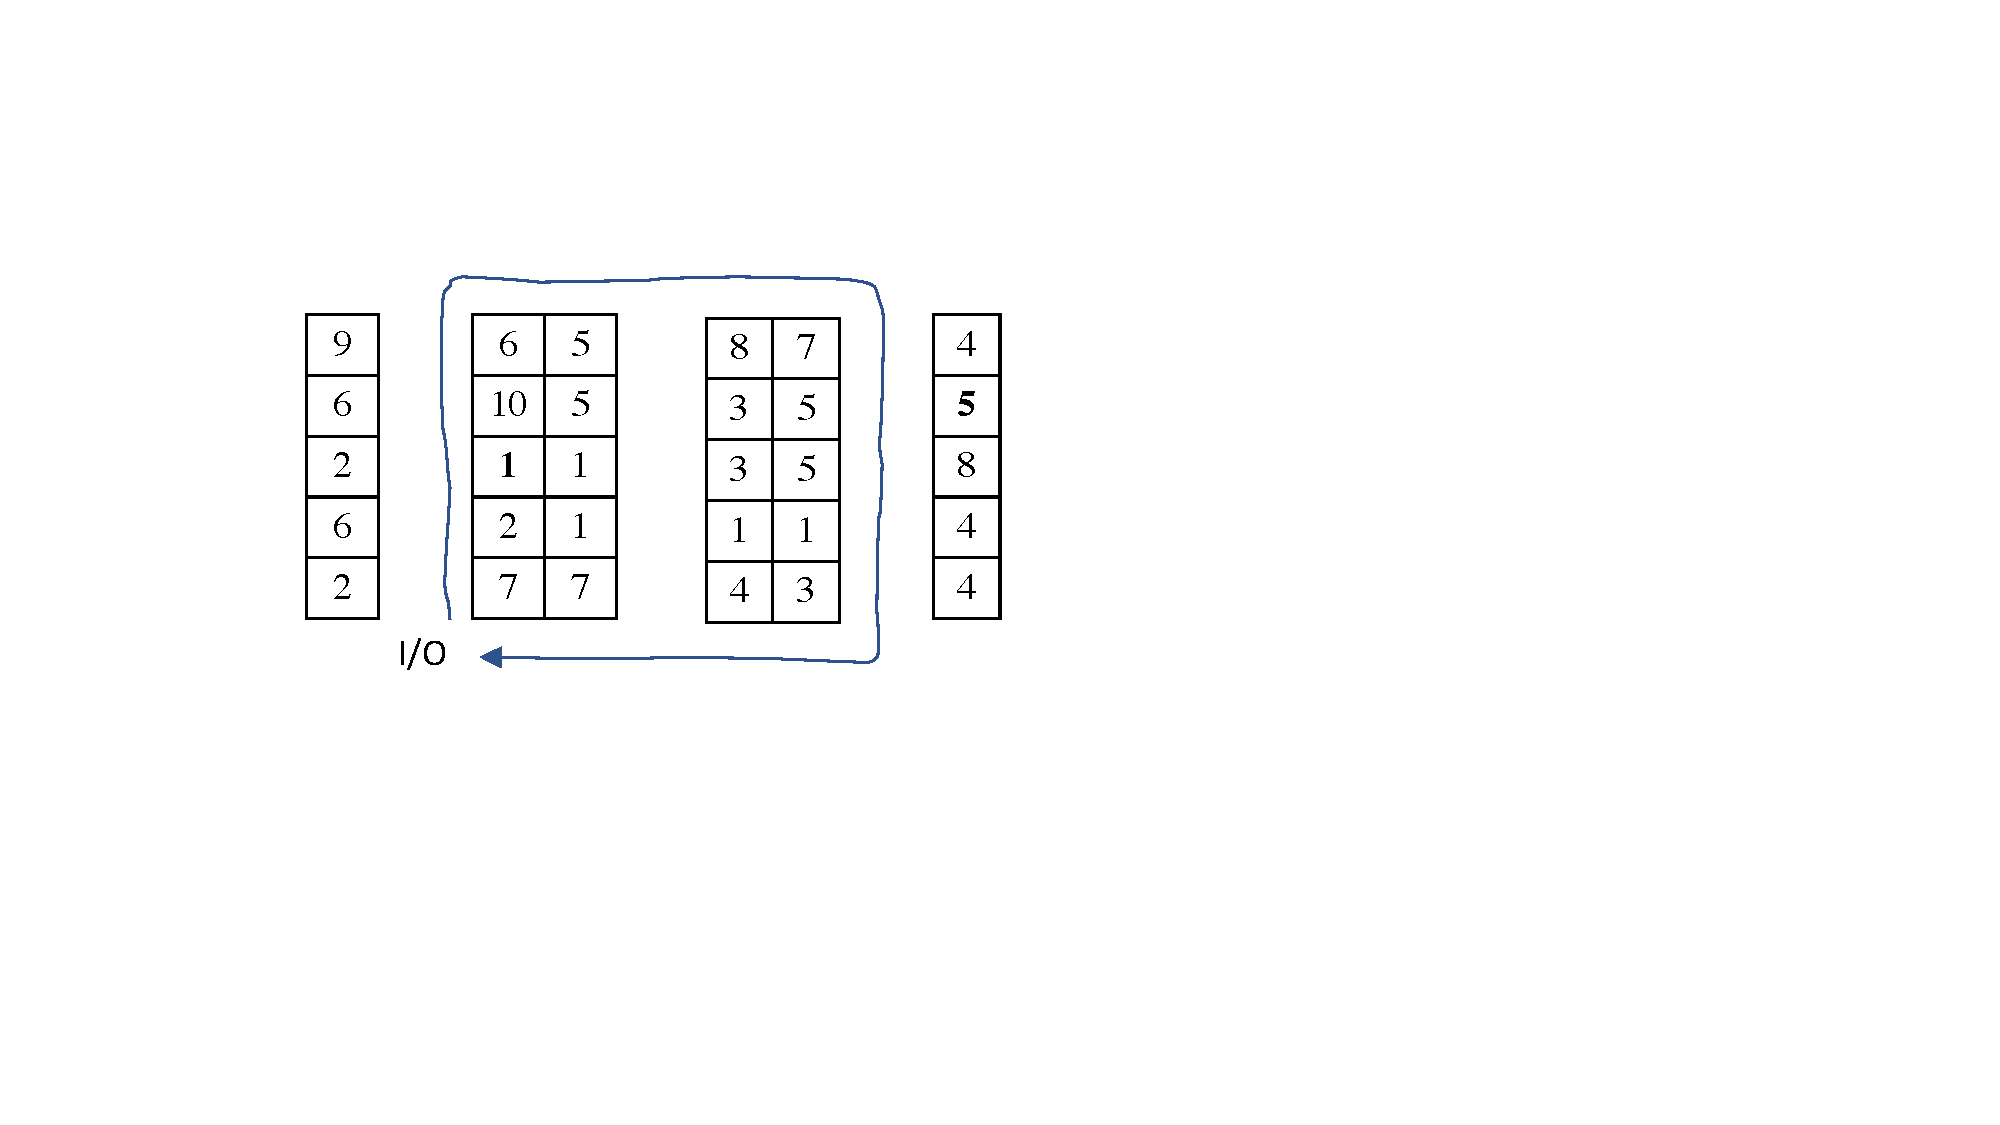
\includegraphics[scale=0.5]{routing}
\centering
\caption{picking 1,5, skipping middle column}
\label{fig:routingskip}
\end{subfigure}
\begin{subfigure}{.5\textwidth}
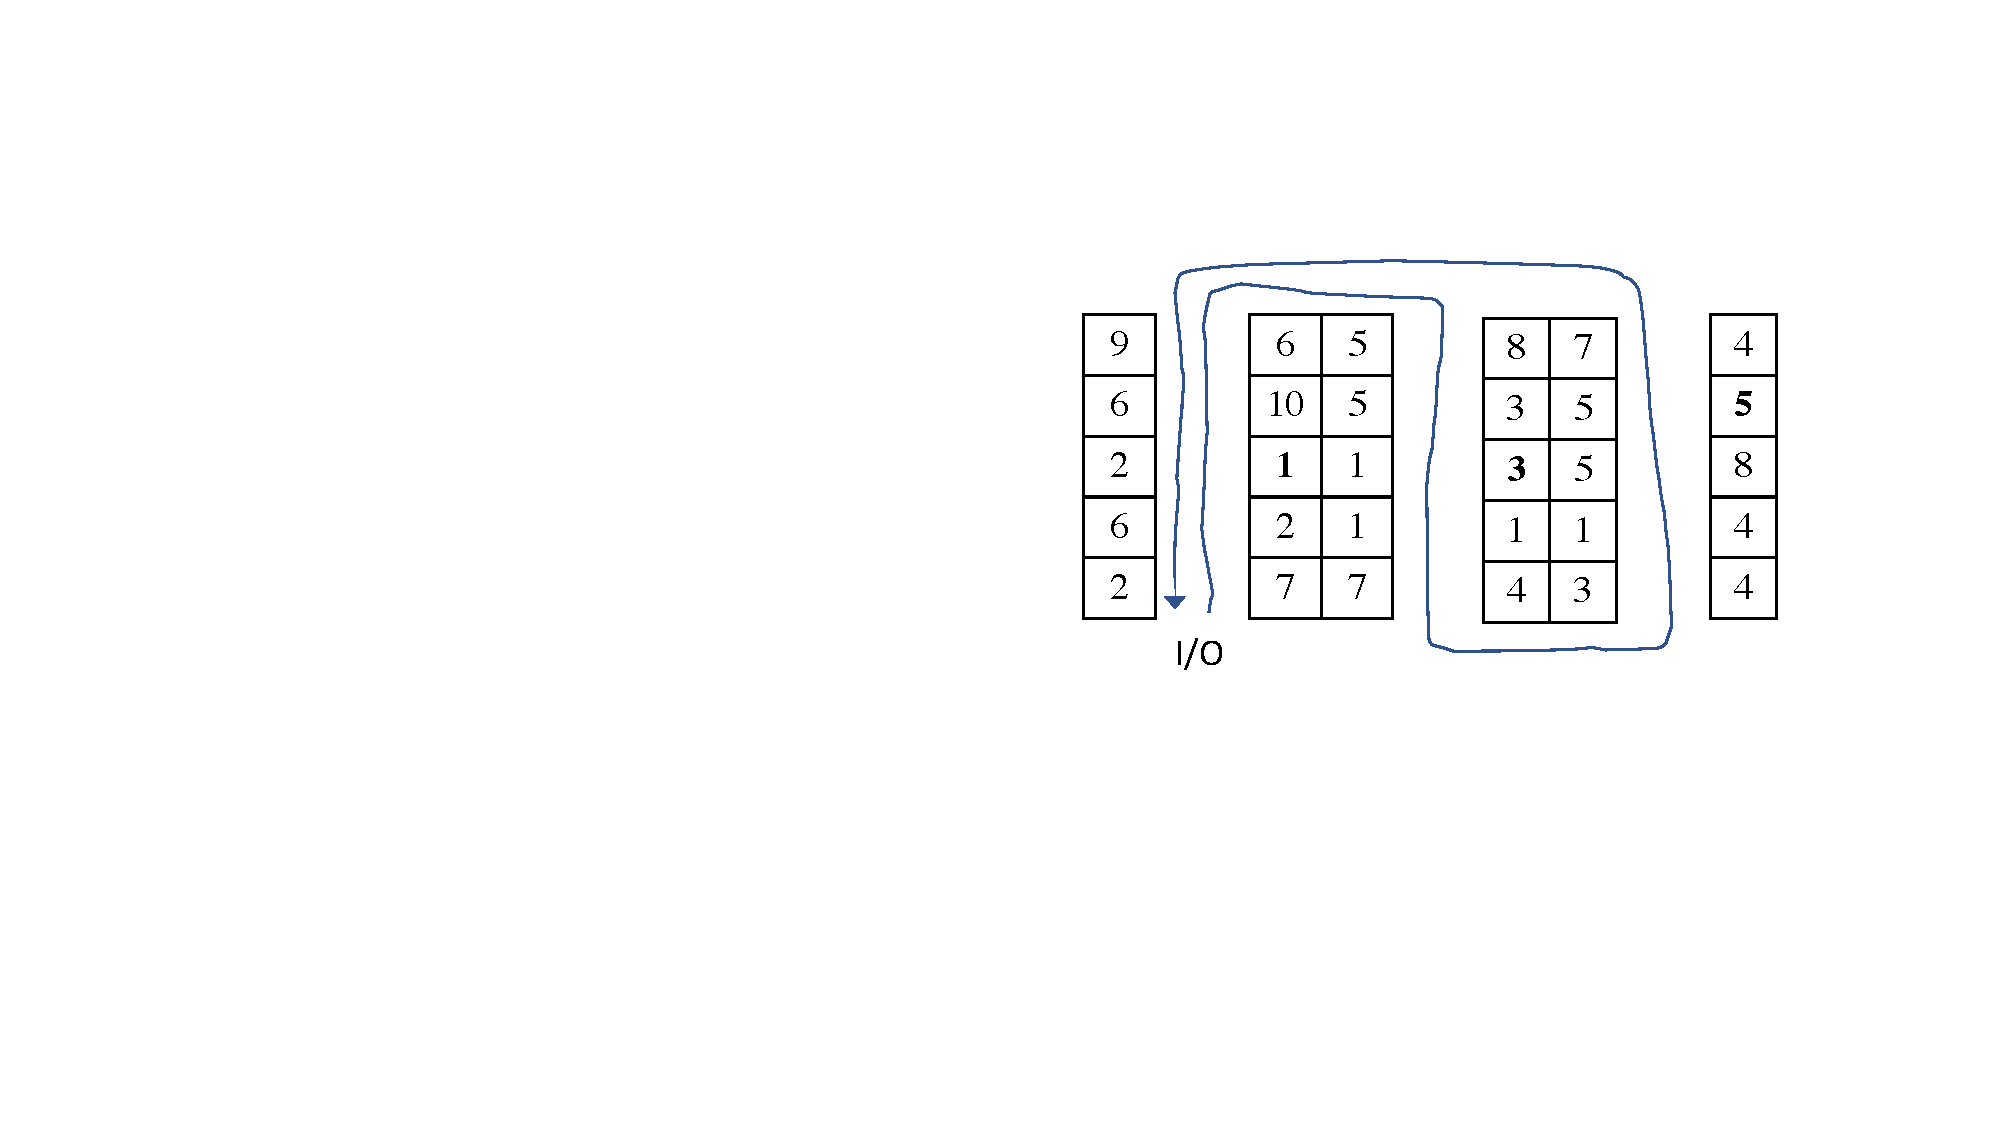
\includegraphics[scale=0.5]{routing2}
\centering
\caption{picking 1,5, not skipping middle column}
\label{fig:routingthrough}
\end{subfigure}
\caption{distances in different situations}
\label{fig:diffdist}
\end{figure}

\textbf{QAP:}

$n$ - \#items = \#locations

$F = (f_{ij})$ - The flow matrix for items. Each entry represents flow between items $i$ and $j$.

$D = (d_{kl})$ - The distance matrix. Each entry represents distance between locations $i$ and $j$.

$X = (x_{ij})$ - The binary decision matrix. Each entry represents whether item $i$ is assigned to location $j$.

Minimise:
\begin{equation}
\sum_{i=1}^{n}\sum_{j=1}^{n}\sum_{k=1}^{n}\sum_{l=1}^{n}f_{ij}d_{kl}x_{ik}x_{jl}\end{equation}

Subject to:
\begin{align}
\sum_{k=1}^{n}x_{ik}=1 \qquad \forall 1\leq i \leq n \\
\sum_{i=1}^{n}x_{ik}=1 \qquad \forall 1\leq k \leq n
\end{align}

Solving for QAP yields a permutation from item set to location set. This solution is reported to give good performance for warehouse optimisation \cite{Mantel:2007}.

\subsection{}

The basic QUBO has the following symbols defined.

$m$		- Number of decision variables

$X'=(x'_i)$ - The decision (column) vector of size $m$ by 1, denoted by $X$

$Q=(q_{ij})$ - A $m$ by $m$ matrix, denoted by $Q$.

$P(x)$	- The penalty polynomial, which corresponds with constraints in the classic QAP.

Next, we minimise the following formula:
\[X'^TQX' + P(x)\]

This formula does not look equivalent to the aforementioned classic formula. However, the classic formula can be converted to QUBO form. Firstly, the decision matrix in classic QAP is flattened to become the decision vector in QUBO. We do this in the traditional way of indexing 2-D arrays. That is, \[\forall i,j, 0\leq i,j \leq n-1 \qquad x'_{i\times n+j} = x_{ij}\]
Note that $m = n\times n$.
Next, the matrix multiplication in the QUBO formula is expanded. The entries of $Q$ can then be constructed to match the classic formula. The way to do this is as follows.

It can be shown that entries of $Q$ can be obtained by manipulating $F$ and $D$. We can flatten them the same way as we do with $X$ and get vectors $\bar{F}$ and $\bar{D}$, both are column vectors of size $n\times n$ by 1. Then we use the following algorithm:

\bigskip
\singlespacing
\begin{algorithm}[H]
\SetAlgoLined
\KwResult{matrix Q for QUBO}
 M = $\bar{F}\bar{D}^T$\;
 Q = new Matrix($n^2\times n^2$)\;
 \For{i in 0 to $n\times n-1$}{
  Temp = new Matrix($n\times n$)\;
  \For{k in 0 to n-1}{
  	\For{l in 0 to n-1}{
		Temp$[k][l]$ = $M[i][k*n+l]$\;
	}
  }
  $pos_x$ = $floor(i/n)$\;
  $pos_y$ = $i\ mod\ n$\;
  Q$[pos_x:pos_x +n][pos_y:pos_y+n]$ = Temp\;
 }
 return Q\;
 \caption{Convert $\bar{F}$ and $\bar{D}$ to Q}
\label{algo1}
\end{algorithm}
\normalspacing
\bigskip

It could be verified that using the above $Q$, the expansion of QUBO formula corresponds with classic QAP, modulo the penalty polynomial in and the second linear term involving $\alpha$ of the classic formula. The exact derivation is given in Appendix A.

Having obtained the formula, simulated annealing can be applied, letting state be the decision matrix/vector and energy be the formula. The Fujitsu Digital Annealer is developed to accelerate simulated annealing. The class of combinatorial optimisation problems it supports is QUBO only. The aim of this project is to develop such a solution framework on DA and apply it to the relevant warehouse.

\section{Report Organization}
Chapter 2 discusses current literature on generic QAP and hardware acceleration of QAP. Chapter 3 elaborates on designing the solution for QAP in the context of warehouse assignment. Chapter 4 presents our implementation of the solution framework on various platforms (currently only the CPU), and covers testing of the solution. Chapter 5 concludes.

\chapter{Related Work}
\label{ch:related}
1. Existing decomposition techniques for QUBO
2. Existing applications of QA/DA
3. Existing theories on block-structured QAP

The method of using QAP to solve warehouse assignment problems has root in Mantel \cite{Mantel:2007}, in which characteristics of a warehouse is first formalised and formulated into an instance of QAP in ILP form. Following this, there are successful attempts in implementing solutions of QAP \cite{Ruijter:2007} using SA and results are favourable in terms of picking distance reduction while being less computationally intensive than techniques with better results. This finding provides empirical impetus for our method.

Some work has been done on accelerating SA with other hardware. The advent of a Multistart algorithm \cite{Marti:2013} for the SA makes the technique amenable to GPU acceleration. Following this theoretical discovery, attempts have been made by \cite{Sonuc:2018} to parallelise the solution of QAP with SA, with good results. The question that follows is this: is it possible to do a comparison between GPU and DA in terms of delay and solution quality, in the task of solving QAP with DA for warehouses?

However, there has been only one account of solving QAP using dedicated annealing hardware. Very recently, Lobe employs the D-wave machine in solving QAP for flight gate assignment. The problem seeks to assign flights to gates such that the total time travelled by passengers in transferring between gates is a minimised. The technique in solving QAP is quantum annealing, which is, roughly speaking, SA performed in the quantum paradigm. 

The work done in this project is relatively new. This is in the sense that yet another piece of new hardware is employed to solve QAP using SA.

\chapter{Experimental Design}
1. Formal QAP, block-structural QAP, decomposition
2. QAP to QUBO conversion, quadratic penalty, external penalty
3. Algorithm outlines

\section{Design issue: Generalising QAP}
\label{sec:generalQAP}
The QAP introduced in chapter 1 is idealistic in the sense that each item is assigned to exactly one location and each location will contain exactly one item. In general this is not the case. The warehouse in this project has 70,000 locations, not all of them necessarily filled. Thus, we need to generalise our QAP to the case where number of locations are greater than number of items.

Both classic QAP and QUBO formulae generalise well for this purpose. The decision matrix $X$ is defined to be rectangular, of size $n \times m$, rather than square. Sizes of $F$ and $D$ will vary correspondingly. The following definitions can be derived.

$m$ - number of locations

$n$ - number of items

$X = (x_{ij})$ - The $n \times m$ decision matrix. Each entry represents whether item $i$ is assigned to location $j$. 

$F = (f_{ij})$ - The $n \times n$ flow matrix. Each entry represents flow between items $i$ and $j$. First row is popularity.

$D = (d_{kl})$ - The $m \times m$ distance matrix. Each entry represents distance between locations $i$ and $j$.First row is distance from I/O.

Next, we minimise the following modified formula:
\[\sum_{i=1}^{n}\sum_{j=1}^{n}\sum_{k=1}^{m}\sum_{l=1}^{m}f_{ij}d_{kl}x_{ik}x_{jl} + \alpha \sum_{i=1}^{n}\sum_{k=1}^{m}f_{0i}d_{0k}x_{ik}\]

Algorithm 1 can still be applied to yield a $Q$ that is now $n\times m$ by $n \times m$.

\section{Design issue: problem size}
\label{sec:coarse}
A practical problem in our approach is problem size. The warehouse we are dealing with has 70,000 locations and 2,800 SKUs. The number of decision variables is quadratic, which means there are over a million variables. DA supports over 8,000 nodes. One node corresponds with one decision variable. There needs to be a way to reduce the number of variables. In the case of \cite{Lobe:2019}, the D-wave system has only 80 nodes, and there are 28,000 decision variables. The strategy is to group the flights into small QAP instances and solve them one by one. In doing this, there are 163 QAP instances, each with at most 16 flights and 16 gates. Splitting is done randomly. There is no a-priori justification for random splitting other than the hope that some degree of optimality can be preserved.

In this project, a similar strategy has to be used for the lack of a more powerful alternative. In the first stage, items are split into bunches. Each bunch makes up one QAP instance with reduced $F$ and $D$ matrices. After solving each instance, there is an aggregation process where an aggregate $F$ is computed between each pair of bunches, and an aggregate $D$ is computed from each pair of (aggregate) locations. These attributes constitute a QAP instance in the second stage which is solved to assign bunches to (aggregate) locations, thus determining the final locations of items. The overall process is named \textit{coarse-grained} QAP.

\subsection{Splitting}
\label{sec:splitting}
Splitting in general is an arbitrary process. A plausible heuristic is that items frequently ordered together should go into the same bunch. It is assumed that each bunch occupies a contiguous area in the warehouse, so items in the same bunch are close to each other. Following this heuristic, the sum of flows should be maximised. The following quantities can be defined:

\begin{tabular}{ll}
$n,m$ & - number of items and locations respectively, as before\\
$b$ & - number of bunches (required to divide $m$)\\
$s = \frac{m}{b}$ &- number of locations for each bunch\\
$F$ &- flow matrix, as before\\
$A = (a_{ij})$ & - binary decision matrix of size $n\times b$, for bunching. Each entry represents whether item $i$ is assigned to bunch $j$
\end{tabular}

The formula to maximise is written as: \[\sum_{k=1}^{b}\sum_{i,j=1}^{n}f_{ij}a_{ik}a_{jk}\]
There are some constraints that need to be satisfied:

\begin{tabular}{ll}
$\sum_{k=1}^{b}a_{ik} = 1 \quad \forall i, 1\leq i\leq n$ & Each item is assigned to only one bunch\\
$\sum_{i=1}^{n}a_{ik} \leq s \quad \forall k, 1\leq k \leq b$ & Each bunch should not exceed capacity\\
\end{tabular}

\bigskip Note that the formula above can also be viewed as a QAP with distance equal to constant 1 and no linear term.

The result of solving the above formula is a decision matrix $A$ indicating which bunch each item belongs to.

\subsection{QAP for individual bunches}
After obtaining the bunches, the generalised QAP formula introduced in section \ref{sec:generalQAP} is applied to determine the relative locations of items within each bunch.

In order to run the minimisation, parameters $F$ and $D$ need to be supplied. First, consider parameter $F$. Note that both matrices need to be individually computed for the bunch. For that purpose, the original flow matrix $F$ can be specialised easily by a lookup procedure. That is, between items $i$ and $j$ of the bunch, their flow is $f_{ij}$, the corresponding entries in $F$. Note that during implementation, a fresh set of indices for items may need to be provided within the bunch, so for each bunch there is a bijective map between the set of bunch-specific indices and the set of original indices.

\begin{figure}
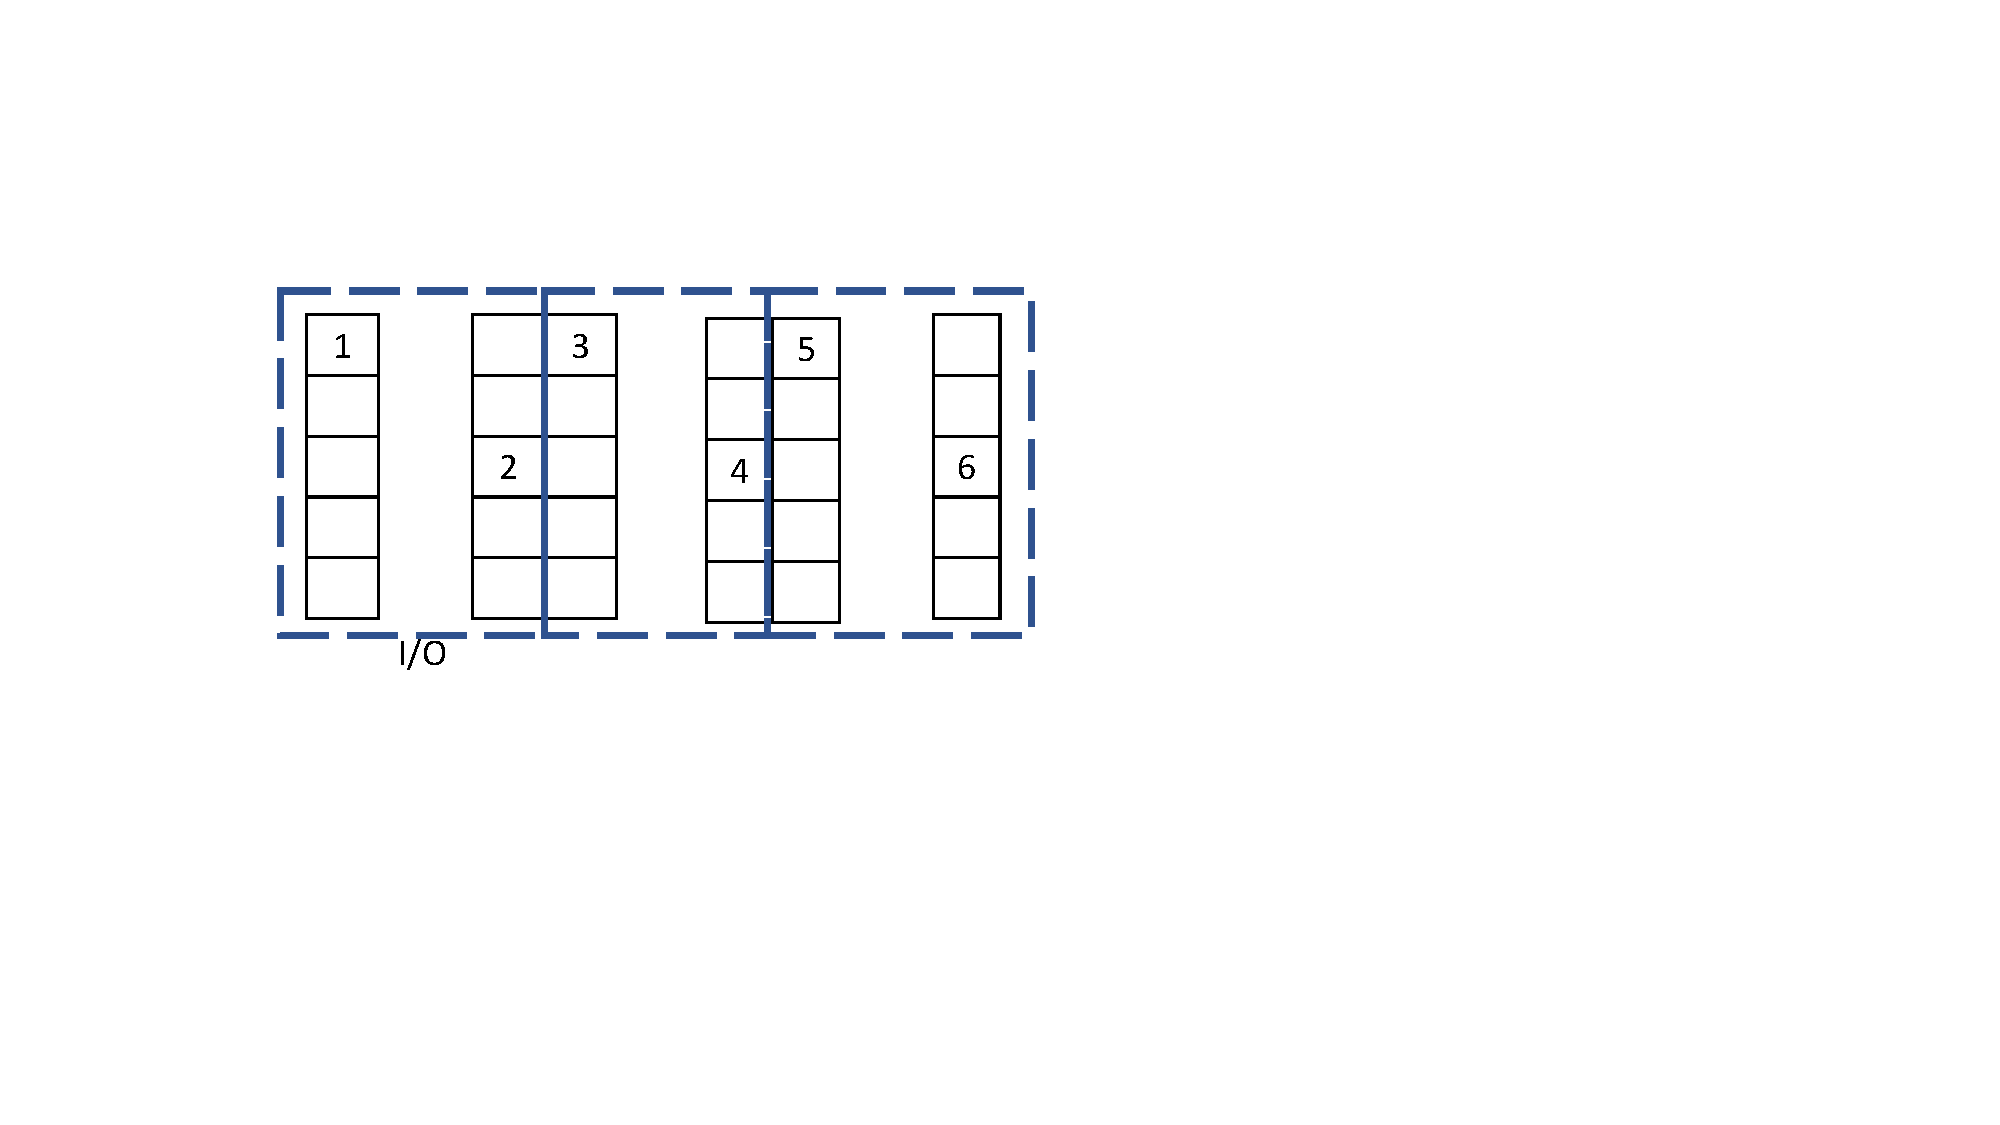
\includegraphics[scale=0.8]{bunches}
\centering
\caption{Areas for bunches}
\label{fig:buncharea}
\end{figure}

Next, consider parameter $D$, the distance matrix within the bunch. Since only relative locations are considered, distance from the I/O point does not matter. Moreover, if the areas for all bunches have a uniform and regular shape such as in Fig \ref{fig:buncharea}, relative distances between corresponding locations for all bunches are identical. For example, in Fig \ref{fig:buncharea}, distances between the pairs of locations (1,2), (3,4), (5,6) are the same. This implies that specifically in situations similar to that of Fig \ref{fig:buncharea}, where all areas have the same shape and size, all bunches share the same distance matrix, so $D$ does not have to be individually computed.

Let the original distance matrix be $D_0$, and the bunch-specific distance matrix be $D$. Assume that distance between each pair of locations is the same whether in $D_0$ or $D$. Then for the distance between locations $i$ and $j$ in $D_0$, the corresponding entry in $D$ (if $i$ and $j$ are in the bunch of $D$, of course) will have the same value as in $D$. Repeating this procedure for each entry in $D$, $D$ can be computed based on $D_0$.

In general, it is inaccurate to assume that distances between two locations are the same whether in $D$ or $D_0$. The following two statements for a short-cut cannot be simultaneously satisfied:\par
1) Between any two locations, their distance in $D$ equals their distance in $D_0$\par
2) $D$ is identical for all bunches\par

\begin{figure}
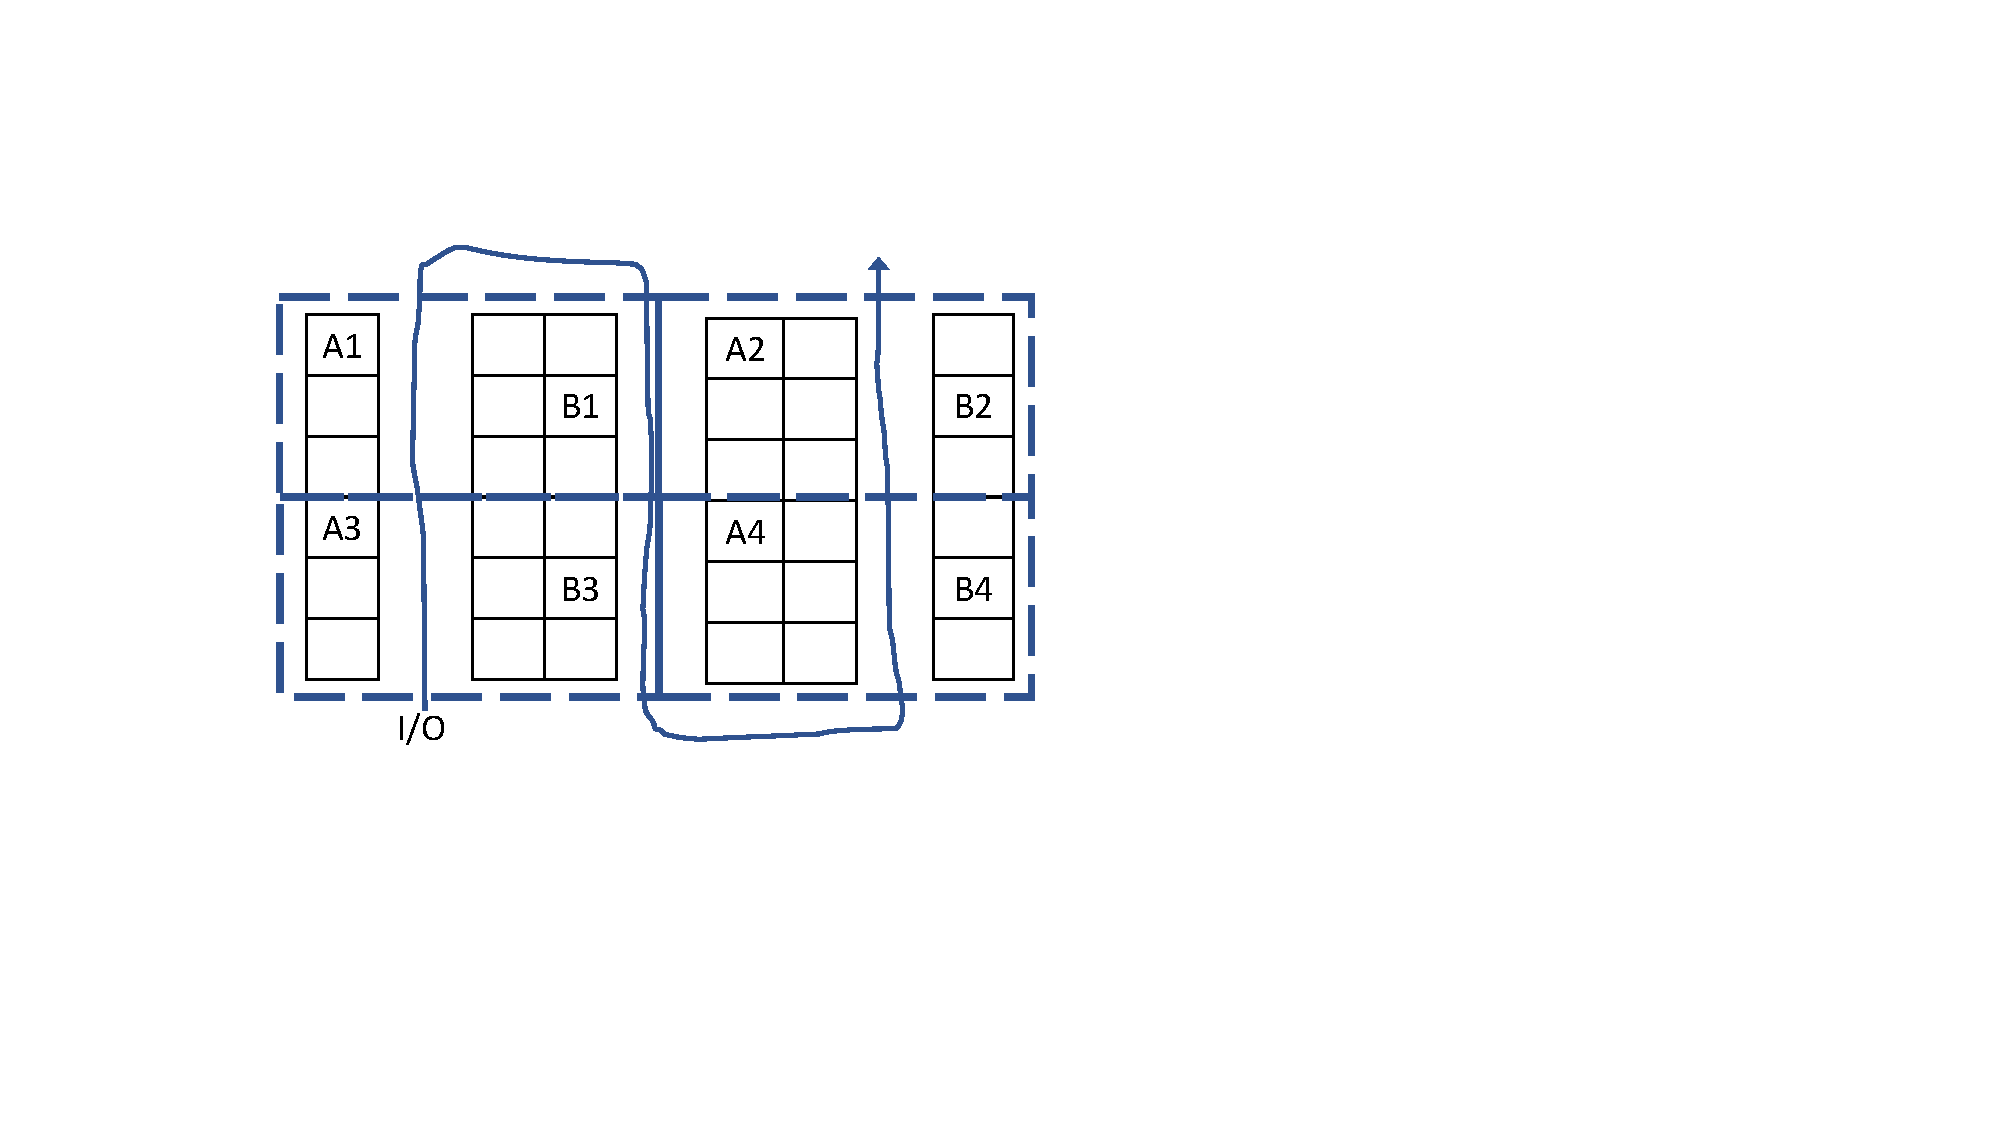
\includegraphics[scale=0.7]{bunches2}
\centering
\caption{A particular area assignment for bunches}
\label{fig:area}
\end{figure}

Consider the areas as shown in Fig \ref{fig:area}. When one bunch occupies different columns, and the route used to compute $D_0$ follows the arrow, it could be seen that distances of different pairs of $(A_i,B_i)$ are different. Therefore, $D$ is not identical across bunches. On the other hand, if $D$ is forced to be the same for all bunches, then it is wrong to compute $D$ by looking up $D_0$, because otherwise $D$ will be different. The cause of this phenomenon is that although bunches have the same shape and size, the aisles crossing them have different structures. For example, the upper left corner has an aisle between the first two columns while the upper right has an aisle between the last two columns.

To avoid this complication, the division of area as shown in Fig \ref{fig:buncharea} is adhered to for all current implementations.

\subsection{QAP for aggregation}
After determining locations of items within each bunch, an aggregation procedure is used to define an abstract \textit{item} out of each bunch. The main motivation for this stage is to account for popularity by placing more popular bunches closer to the I/O point, since only relative locations have been considered in previous stages. Additionally, if two bunches have items that are more frequently ordered together, the two bunches should be closer to each other as well.

The aggregate properties are defined as follows. Conceptually, flow means how often items are ordered together. Thus, flow of two bunches can be defined as the sum of flows between each combination of two items from the two bunches respectively. That is, for bunches $A$ and $B$, 
\[F_{AB} = \sum_{i=1}^{s}\sum_{j=1}^{s}f_{ij}\]
\[F_{0k} = F_{k0} = \sum_{l=1}^{s}f_{0l}\]
where $i$ ranges the items from bunch A and $j$ ranges those from bunch B. Moreover, the popularity of each bunch is defined as the sum of popularity of items in the bunch, and is reflected in the first row of $F$. Overall, $F$ is $(b+1) \times (b+1)$, where $b$ is number of bunches as defined in section \ref{sec:splitting}. \par
The aggregate distance between two big locations is defined in the Euclidean way, since it does not make sense speaking about S-shape routing while dealing with bunches. In Fig \ref{fig:buncharea} each bunch is regarded as a point, so there are in total 3 points, say $a, b, c$ from left to right. Then the distances are given as\bigskip

\begin{center}
\begin{tabular}{|c|c|c|c|c|}
\hline
$D$ & $0$ & $a$ & $b$ & $c$\\
\hline
$0$ & $0$ & $1$ & $2$ & $3$\\
\hline
$a$ & $1$ & $0$ & $1$ & $2$\\
\hline
$b$ & $2$ & $1$ & $0$ & $1$\\
\hline
$c$ & $3$ & $2$ & $1$ & $0$\\
\hline
\end{tabular}
\end{center}

\bigskip Let the bunches be named 1,2,3. The decision matrix $X_{3\times 3}$ is defined as $x_{ij}$ - whether bunch i is allocated to location j. Here, i ranges from 1 to 3 while j ranges from $a$ to $c$.

This way, all parameters for a final QAP is defined. The QAP formula as introduced in \ref{sec:qap} can be instantiated and solved. The solution will be an arrangement of bunches, which can be interpreted to give the final locations of all items in the warehouse.

\chapter{Evaluation}
1. System setup
2. dataset
3. Methodology
4. Results

Fujitsu has not provided us with DA access, and the company has not provided us with data. Thus, we reproduce the example introduced in Section \ref{sec:example} as a preliminary test of the quality of the coarse-grained QAP formula.

\section{Implementation}
The platform for the initial implementation is IBM ILOG Optimisation Studio that runs on Intel X86 i5 CPU. There are three stages as introduced in section \ref{sec:coarse}. All QAP formulae are implemented in ILOG, while data manipulation is done with Python that interacts with the software via the file system.

The high-level procedure of the implementation has the following steps.\par
1) Create order set, store in file\par
2) Parse order set from file, generate $F$\par
3) Specify shape of warehouse and generate $D$\par
4) Run grouping.mod, the ILOG model for splitting\par
5) Extract the bunches from step 4) and run warehouse.mod, the ILOG model for generic QAP for each\par
6) Generate aggregate $F$ and $D$ and run warehouse.mod again. The locations of items are finalised after this step.

In subsequent sections, some key elements of the above procedure are described. In particular, the two ILOG models are covered. There is a fair amount of utility code in Python for generating the various matrices in steps 2,3,5 and 6. This is not discussed here and the full code is uploaded to https://github.com/willxujun/QUBO for reference.

\subsection{warehouse.mod}
In ILOG, the representation of decision variable is slightly different from the classic QAP. A linear array \textit{perm}, of length $m$, the number of locations is used. Each entry in the array represents an indexed location, where the index is just the array's index. SKUs are represented as numbers from 1 to n. An array entry could be 0 or any number between 1 to n. 0 means the location is empty and non-zero $i$ represents the location is assigned some item of SKU $i$. $F$ and $D$ are defined as before. The entire cost function, the formula to be minimised, is the following:
\begin{verbatim}
cost = 
 	sum(ordered i,j in LOCS1)
 		(perm[i]!=0)*(perm[j]!=0)*F[perm[i]][perm[j]]*D[i][j]
 	+ sum(i in LOCS1)
 		F[0][perm[i]]*D[0][i]
 	;
\end{verbatim}
where LOCS1 is the set of indices for locations. The idea is to make array references instead of relying on expanded binary matrices. Definitionally, the above representation is not the same as the original, but denotationally they are the same quantity. The motivation of doing this is to leverage the expressiveness of software. In later stages of this project, the representation will have to be translated to QUBO form and implemented elsewhere.

Additionally, the constraints are expressed as follows:
\begin{verbatim}
number_of_zeros:
 count(all(i in LOCS1) perm[i],0) == NUM_LOCS - sum(i in SKUS) qty[i];
number_of_items:
 forall(x in SKUS)
 	count(all(i in LOCS1) perm[i],x) == qty[x];
\end{verbatim}

The array \textit{qty} is gleaned from the order set, indexed by number of SKUs, that expresses how many items there are for each SKU. Thus, the first constraint expresses that the number of zeros in the decision array \textit{perm} is the number of unoccupied locations. The second constraint restricts the number of items to what is specified by \textit{qty}. Noticeably, these constraints are different from the one introduced in section \ref{sec:qap} due to different representations. In section \ref{sec:qap}, there is no need to restrict the number of items on the decision matrix because it has been pre-computed and embodied in the size of the matrix. In warehouse.mod, there is no need to worry about unique location for each item because each entry of \textit{perm} can only contain one number.

Note that this implementation can be used to solve all QAP in its most generalised form, as introduced in section \ref{sec:generalQAP}. To use this package, one simply needs to supply $F$, $D$ and specify the numbers of items and locations.

\subsection{grouping.mod}
There is a separate implementation \textit{grouping.mod} that contains the model for the initial splitting process. The decision variable is \textit{grouping}, an $n\times b$ 2-dimensional binary array. The expression of flow, corresponding with the formula in section \ref{sec:splitting}, together with constraints, is as follows.
\begin{verbatim}
flow = 
 	sum(s in GROUPS)
 		sum(ordered i,j in ITEMS)
 		  F[item_to_sku[i]][item_to_sku[j]]*grouping[i][s]*grouping[j][s];

//every item is assigned to only 1 group
ct1:
 	forall(x in ITEMS)
 	 count(all(s in GROUPS) grouping[x][s], 1) == 1;
 	 	
//every group contains less than or equal to group_size items
ct2:
 	forall(s in GROUPS)
 	 count(all(i in ITEMS) grouping[i][s], 1) <= group_size;
\end{verbatim}

Full code for the two .mod files is given in Appendix B.

\section{Results}
Fig \ref{fig:coarselayout} shows the output for coarse-grained QAP. The algorithm behind the optimisation studio is not available, and is unlikely to be simulated annealing. However, splitting and aggregation QAP can finish within seconds. QAP for each bunch was allowed to run for 600 seconds. Computation time is not significant at present because 1) the dataset is not the actual one and 2) there is no benchmark to compare it with. Perhaps when other platforms become available, such as GPU or DA, this result will have more value.

\begin{figure}
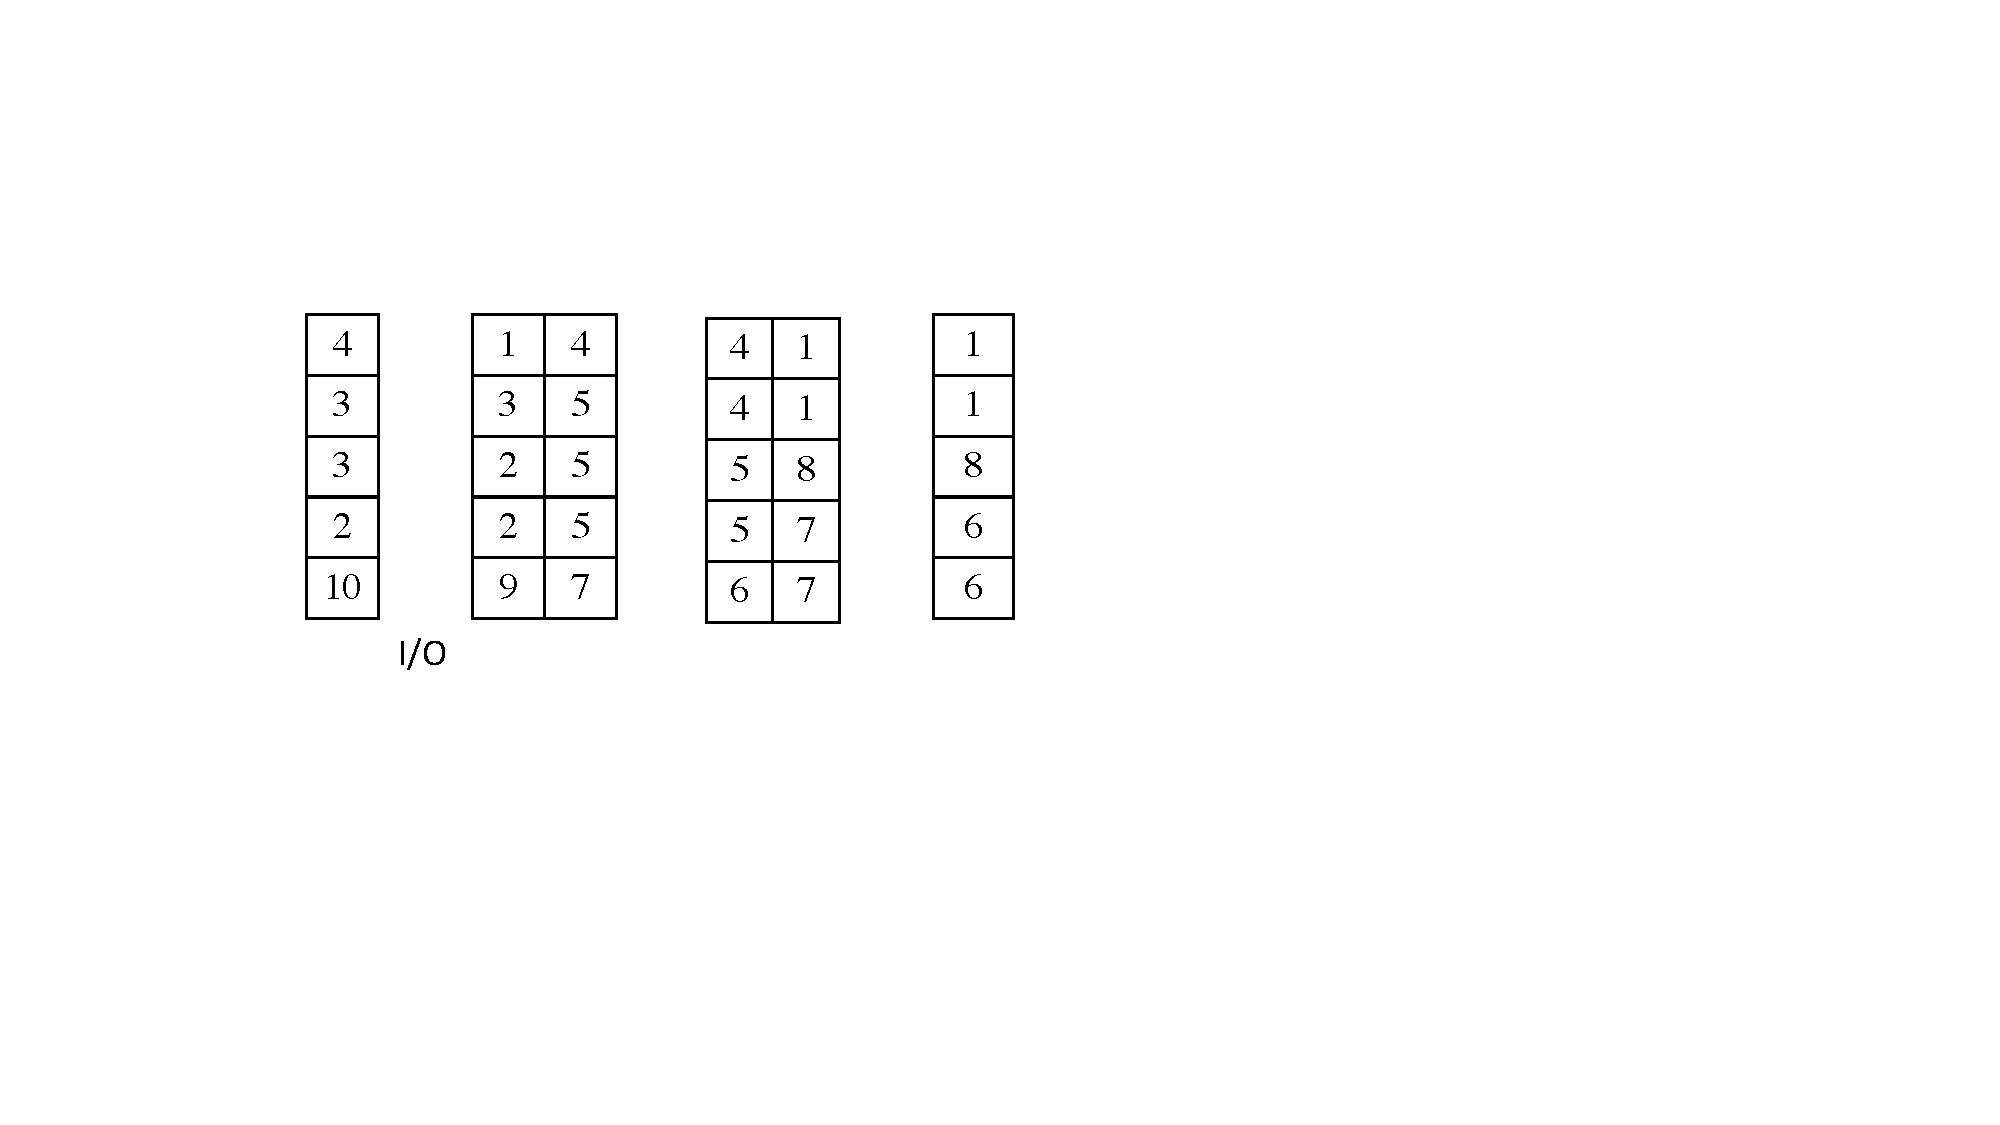
\includegraphics[scale=0.8]{me}
\centering
\caption{layout generated by coarse-grained QAP}
\label{fig:coarselayout}
\end{figure}

A verification exercise is done manually to evaluate the various solutions in Fig \ref{fig:variouslayouts} as well as Fig \ref{fig:coarselayout}. The order set follows Fig \ref{fig:orderset}. It is assumed that crossing each storage location vertically, within the same aisle, is 1 unit distance. Traversing an entire aisle is 6 units distance. Changing aisle horizontally takes 3 units distance. The result is shown in table \ref{tbl:result}. It could be seen that for this example, coarse-grain QAP performs equally well as order-oriented swapping, which is the simulated annealing strategy that computes traversed distance with brute force. Both OOS and coarse-grain QAP has 22 vertical aisle traversals and 32 horizontal aisle change, the lowest among all strategies. This is a promising result that validates the potential of coarse-grain QAP in solving realistic warehouse situations.
\begin{table}[h]
\centering
\begin{tabular}{|c|c|c|c|}
\hline
Strategy & \#vertical traversal & \#horizontal aisle change & total distance\\
\hline
COI	& 28 & 34 & 270\\
\hline
Random & 26 & 32 & 252\\
\hline
ABC & 24 & 36 & 252\\
\hline
OOS & 22 & 32 & 228\\
\hline
coarse-grain QAP & 22 & 32 & 228\\
\hline
\end{tabular}
\caption{Distances traversed in picking order set for various strategies}
\label{tbl:result}
\end{table}

Verification by hand is not realistic as dataset gets large. Therefore, work is in progress to build a simulator that takes routing strategy, assignment strategy and order set as input and outputs total distance travelled.

\chapter{Conclusion}
1. ...

Coarse-grain QAP is promising in solving warehouse assignment problems. In particular, the advantage of using this technique, as seen from the example of the current stage, is the preservation of solution quality, while enabling acceleration on application-specific hardware. On paper, QAP also has low computational cost, but this has not manifested because of lack of equipment access. Hopefully, when DA and actual data are provided, the full-scale implementation will yield equally high-performing solutions.

\section{Future Work}
Firstly, distance modelling is the most difficult part of the project so far. The QAP requires a priori distance between any two items in order to effectively minimise traffic, and yet distance between two items is often not very clear. There are two reasons for this. The first reason is routing policy, which will result in different distances between two items even within the same order set. The second reason is the complication which arises from the coarse-grain technique. The concept of routing-specific distance is blurred when considering separate bunches of items because routing does not sensibly apply within a bunch. Moreover, choice of areas will also affect distances.

In light of the above discussion, the aim of future work is to model distance more accurately. Some generic notion of proximity is desired to accurately measure the actual \textit{closeness} between any two locations when items are picked, so that QAP can model more realistic picking situations.

Secondly, another area worthy of exploring is acceleration on GPU. This is to provide a basis with which DA's performance can be compared.

Thirdly, coarse-grain QAP is primarily a heuristic technique. It is employed because there is currently no better way of reducing the number of binary decision variables for running QAP on DA. While this works out well in the example, some formal, a-priori justification is desired to guarantee the preservation of solution quality on realistic datasets.

\bibliographystyle{socreport}
\bibliography{example}

\appendix
\chapter{Derivation of QUBO formula}
Let $X$ be the $n \times m$ decision matrix in the original QAP formula. Let $F$ be the $n\times n$ flow matrix, with the first row and the first column both representing popularity of an item. Let $D$ be the $m\times m$ distance matrix with the first column and the first row both representing distance from I/O point. Note that $F$ and $D$ are symmetric and $n\leq m$. Recall the quadratic part of the classic QAP formula,
\[\sum_{i=1}^{n}\sum_{j=1}^{n}\sum_{k=1}^{m}\sum_{l=1}^{m}f_{ij}d_{kl}x_{ik}x_{jl} \qquad (1)\]
the goal is to show that (1) is equivalent to
\[\vec{x}^TQ\vec{x}\]
for some matrix $Q$ of size $nm\times nm$ and some decision vector $\vec{x}$.\par
Let $\vec{x}_{(i-1)\times m + j} = x_{ij}$.
\singlespacing
Let $Q = \begin{pmatrix}q_1&q_2&...&q_{nm}\end{pmatrix}$, where $q_i$ are columns of $Q$.
\begin{equation}
\begin{split}
\vec{x}^TQ\vec{x} & = \vec{x}^T \begin{pmatrix}q_1&q_2&...&q_{nm}\end{pmatrix} \vec{x} \\
				  & = \begin{pmatrix}\vec{x}^Tq_1&\vec{x}^Tq_2&...&\vec{x}^Tq_{nm}\end{pmatrix}\vec{x} \\
				  & = \vec{x}^Tq_1x_1 + \vec{x}^Tq_2x_2  + \vec{x}^Tq_{nm}x_{nm}\\
				  & = \sum_{i=1}^{n}\sum_{j=1}^{n}\sum_{k=1}^{m}\sum_{l=1}^{m}x_{ik}q_{((i-1)m+k)((j-1)m+l)}x_{jl} \\
\end{split}
\end{equation}
Comparing with the original formula, we have
\[f_{ij}d_{kl} = q_{((i-1)m+k)((j-1)m+l)}\qquad (2)\] 
Next we flatten $F$ and $D$.
Let $\vec{f}_{(i-1)\times n + j} = f_{ij}$, $\vec{d}_{(i-1)\times m + j} = d_{ij}$.

\begin{equation}
\begin{split}
\vec{f}^T\vec{d} & = \begin{pmatrix}f_{11}\\f_{12}\\...\\f_{nn}\end{pmatrix}
					\begin{pmatrix}d_{11} & d{12} & ... & d_{nn}\end{pmatrix} \\
				& = \begin{pmatrix}
					f_{11}d_{11} & f_{11}d_{12} & ... & f_{11}d{mm} \\
					f_{12}d_{11} & f_{12}d_{12} & ... & f_{22}d{mm} \\
					\vdots 		 & & & \vdots \\
					f_{nn}d_{11} & f_{nn}d_{12} & ... & f_{nn}d{mm} \\
					\end{pmatrix}
					\\
				& = \begin{pmatrix}
					q_{11} 	   				 & q_{12}     & ... & q_{mm} \\
					q_{1(1+m)} 				 & q_{1(m+2)} & ... & q_{m(m+m)} \\
					\vdots 	   				 &            &     & \vdots \\
					q_{((n-1)m+1)((n-1)m+1)} & 			  & ... & q_{(nm)(nm)} \\
					\end{pmatrix} \qquad (3)
\end{split}
\end{equation}
\normalspacing

Noticeably, each row in (3) is a small, square sub-matrix of $Q$ of size $m\times m$. The upper left corner of the sub-matrix is specified by the start of the row, and the entries of the sub-matrix are filled row-by-row, scanning the row of (3) from left to right. This is exactly what is done in Algorithm \ref{algo1}.

Incorporating the linear term of classic QAP formula into QUBO form can be done by adding the constant $\alpha$ to the beginning of $\vec{x}$. Accordingly, $Q$ has to be adjusted to meet this requirement. In particular, it will expand by 1 to become size $(nm+1)\times(nm+1)$, and the first column will become the linear terms as computed from the 0th rows of $F$ and $D$. The detail is very technical and is omitted.
\chapter{Code of ILOG models}
\section{grouping.mod}
\singlespacing
\begin{verbatim}
using CP;

 int group_size = 10;
 int num_skus = 10;
 range SKUS = 1..num_skus;

 range frange = 0..num_skus;
 int F[frange][frange] = ...;
 
 int num_items = sum(i in SKUS) F[0][i];
 int num_groups = ftoi(ceil(num_items / group_size));
 
 range ITEMS = 1..num_items;
 int item_to_sku[ITEMS];
 
 execute {
 	var a = 1;
  	for(var i in SKUS) {
  	  	for(var s=1; s<=F[0][i]; s++) {
  	  		 item_to_sku[a] = i;
  	  		 a+=1;	  	
  	  	}
  	}
 }
 
 range GROUPS = 1..num_groups;

 dvar boolean grouping[ITEMS][GROUPS];
 
 dexpr int flow = 
 	sum(s in GROUPS)
 		sum(ordered i,j in ITEMS)
 		  F[item_to_sku[i]][item_to_sku[j]]*grouping[i][s]*grouping[j][s];
 maximize 
 	flow
 	;
 subject to {
 	 //every item is assigned to only 1 group
 	 ct1:
 	 forall(x in ITEMS)
 	 	count(all(s in GROUPS) grouping[x][s], 1) == 1;
 	 	
 	 //every group contains less than or equal to group_size items
 	 ct2:
 	 forall(s in GROUPS)
 	 	count(all(i in ITEMS) grouping[i][s], 1) <= group_size;
 }
 
\end{verbatim}
\normalspacing

\section{warehouse.mod}
\singlespacing
\begin{verbatim}
using CP;

 int NUM_SKUS = ...;
 int NUM_LOCS = ...;
 range SKUS = 1..NUM_SKUS;

 range drange = 0..NUM_LOCS;
 range frange = 0..NUM_SKUS;

 int F[frange][frange] = ...;
 int D[drange][drange] = ...;
 int qty[frange] = ...;
 
 execute {
 	cp.param.timeLimit=60;
 	writeln(D);
 	writeln(F);
 	writeln(qty);
 }

 range LOCS1 = 1..NUM_LOCS;
 range assignment = 0..NUM_SKUS;
 dvar int perm[LOCS1] in assignment;
 
 dexpr int cost = 
 	sum(ordered i,j in LOCS1)
 		(perm[i]!=0)*(perm[j]!=0)*F[perm[i]][perm[j]]*D[i][j]
 	+ sum(i in LOCS1)
 		F[0][perm[i]]*D[0][i]
 	;
 
 minimize
 	cost;
 	
 subject to {
 	
 	number_of_zeros:
 	count(all(i in LOCS1) perm[i],0) == NUM_LOCS - sum(i in SKUS) qty[i];

	number_of_items:
 	forall(x in SKUS)
 	  count(all(i in LOCS1) perm[i],x) == qty[x];
 	 
 }
\end{verbatim}
\normalspacing
\end{document}
